\documentclass{report}
\usepackage{setspace}
\usepackage{bookmark}
%\usepackage{subfigure}

% my extra package imports;
\usepackage{caption}
\usepackage{algpseudocode}
\usepackage{algorithm}
\usepackage{float}
\usepackage{hyperref}
\usepackage{subcaption}
\usepackage{graphicx}
\usepackage{graphics}
\usepackage{tikz}
\usetikzlibrary {positioning, shapes, bayesnet}
\graphicspath{{./}}
\usepackage{natbib}

\usepackage[top=2.5cm, left=3cm, right=3cm, bottom=4.0cm]{geometry}                                                                                      
% Colour table cells
% \usepackage[table]{xcolor}
% Get larger line spacing in table
% \newcommand{\tablespace}{\\[1.25mm]}
% \newcommand\Tstrut{\rule{0pt}{2.6ex}}         % = `top' strut
% \newcommand\tstrut{\rule{0pt}{2.0ex}}         % = `top' strut
% \newcommand\Bstrut{\rule[-0.9ex]{0pt}{0pt}}   % = `bottom' strut
% end of my imports;
\pagestyle{plain}
\usepackage{amssymb,color}
\usepackage{amsfonts}
\usepackage{latexsym}
\usepackage{a4wide}
\usepackage{amsmath}

\newtheorem{theorem}{THEOREM}
\newtheorem{lemma}[theorem]{LEMMA}
\newtheorem{corollary}[theorem]{COROLLARY}
\newtheorem{proposition}[theorem]{PROPOSITION}
\newtheorem{remark}[theorem]{REMARK}
\newtheorem{definition}[theorem]{DEFINITION}
\newtheorem{fact}[theorem]{FACT}

\newtheorem{problem}[theorem]{PROBLEM}
\newtheorem{exercise}[theorem]{EXERCISE}
\def \set#1{\{#1\} }

\newenvironment{proof}{
PROOF:
\begin{quotation}}{
$\Box$ \end{quotation}}



\newcommand{\nats}{\mbox{\( \mathbb N \)}}
% \newcommand{\rat}{\mbox{\(\mathbb Q\)}}
\newcommand{\rats}{\mbox{\(\mathbb Q\)}}
\newcommand{\reals}{\mbox{\(\mathbb R\)}}
\newcommand{\ints}{\mbox{\(\mathbb Z\)}}

%%%%%%%%%%%%%%%%%%%%%%%%%%

% COVER PAGE;
\title{
  { \includegraphics[scale=.5]{ucl_logo.png}}\\
  {{\Huge Graph style transfer using Inverse Reinforcement Learning}}\\
  % {\large An application to subway networks}\\
}

\date{Submission date: 11 September 2023}
\author{
  Candidate Number: YLLK3\thanks{
      {\bf Disclaimer:}
      This report is submitted as part requirement 
      for the MSc Machine Learning at UCL. It is
      substantially the result of my own work except 
      where explicitly indicated in the text.
      The report may be freely copied and 
      distributed provided the source is explicitly acknowledged.
    }
    \\ \\
  MSc Machine Learning\\ \\
  Supervisors: Prof. Steve Hailes, Prof. Mirco Musolesi, Dr. Victor-Alexandru Darvariu
}

\numberwithin{equation}{section}
\numberwithin{figure}{section}
\numberwithin{table}{section}  
\numberwithin{algorithm}{section}

%%%%%%%%%%%%%%%%%%%%%%%%%%%%%%%%%%%%%%%%%%%%%%%%%%%%%%%%%%%%%%%%%%
% START DOCUMENT;
\begin{document}
\onehalfspacing
\maketitle

%%%%%%%%%%%%%%%%%%%%%%%%%%%%%%%%%%%%%%%%%%%%%%%%%%%%%%%%%%%%%%%%%%
% ABSTRACT;
\begin{abstract}
  \textbf{I THINK THIS IS DONE}


  In this report we investigate methods for learning a graph 
  construction mechanism based on a single graph example. We 
  tackle this problem from the angle of Maximum-Entropy (MaxEnt) 
  Inverse Reinforcement Learning 
  (IRL) whose goal is to learn a reward function given 
  expert demonstrations. 
  
  After learning a reward function, we use it as an 
  objective on a different graph and learn a 
  new policy to perform style-transfer.  
  The style-transfer constitutes transferring the topological 
  propoerties of the source graph to the target graph, while 
  preserving the vertex set attributes of the target graph.
  
  We investigate different ways to achieve this and 
  propose improvements over current methods with respect 
  to decreasing the variance during training of the IRL procedure. 
  These improvements are inspired by the 
  literature on per-decision importance samples 
  in Reinforcement Learning, exploiting conditional independence 
  properties of rewards given states and actions.
  
  In our experiments, we test two ways to achieve style-transfer 
  on graphs. First, we try  
  directly deploying the 
  jointly learned (together with the reward)  
  policy from IRL based on the source graph, 
  on the target graph. Second, 
  we train 
  a new policy on the target graph using the learned reward 
  function from IRL and then sample trajectories from it. 
  In all experiments, we use GraphOpt as our baseline. 
\end{abstract}
\tableofcontents
\setcounter{page}{1}

%%%%%%%%%%%%%%%%%%%%%%%%%%%%%%%%%%%%%%%%%%%%%%%%%%%%%%%%%%%%%%%%%%
% NEW CHAPTER - INTRODUCTION;
\chapter{Introduction and Related Work}\label{chap:intro}
\textbf{I THINK THIS IS DONE;}

As more and more graph data become available, researchers in 
areas such as biology \citep{VGAEDisease}, quantum chemistry 
\citep{MPNNs}, social networks \citep{SocialNets} and others 
seek ways to analyse these data in a way that extracts 
maximum information 
and requires the least amount of hand-designed features.

When it comes to automatic feature-selection, Deep Learning (DL)
is among the most successful paradigms spanning domains like 
text \citep{textCNN,RNNs,SentimentRNN,BERT}, 
vision \citep{alexnet}, and even graphs \citep{ScarselliGNN,VGAE,GCN,GAT}.

The ability of DL to extract predictive features, and generaly 
arrive at continuous embeddings of abstract data types, makes 
it a prominent component of current Deep Graph Learning techniques.

Although methods such as ``node2vec'' and ``DeepWalk'' 
\citep{node2vec,DeepWalk} have been 
proposed to automatically learn node features based on random 
walks over the graph (ignoring node features), 
it has been shown that Graph Neural Networks 
(GNN) \citep{ScarselliGNN,GCN} achieve superior performance in domains 
such as citation graphs \citep{VGAE} and Disease-gene link prediction 
(DGP) \citep{VGAEDisease}, among others. 
It has been postulated that this is because 
of the way GNNs utilise node features during the (neural) 
message passing procedure. Unsurprisingly, this has sparked interest 
in engineering different architectures for neural message passing 
\citep{GCN,MPNNs,GAT,GATv2}.

Outside of prediction, there exist other graph tasks that may be 
of interest such as graph construction. Having access to a 
graph-generative mechanism allows 
one to create synthetic data from a given distribution, which can 
be used for data augmentation, for example. 

Graph-style transfer, is another 
venue of interest, where given a generative mechanism for 
a source graph, one can apply the same on a target graph in order 
to induce structure similar to that of the source graph. The 
last mentioned task is somewhat similar to Neural Style Transfer (NST) 
\citep{NSTGatys} from the computer vision literature, where we 
have a ``content'' image and a ``style'' image. The goal in NST 
is to transfer artistic traits of the ``style'' image 
(e.g., color or style of painting) to the ``content'' image 
while preserving the entities seen in the ``content'' image. In 
the graph setting, we can think of the style as the topology, 
while the content are the nodes (or node features).  

While many prediction tasks, such as edge and/or node-attribute 
prediction \citep{GCN,VGAE,VGAEDisease,node2vec,DeepWalk}, 
have been successfully tackled, 
the area of graph construction has only recently gained popularity 
\citep{Darvariu,DeepMindGraphGen,GCNPolicyGraphGen,GraphRNN,GraphOpt,olivecrona2017molecular,Yang2017}.
Some methods 
utilise probabilistic formulations of the graph generative 
procedure \citep{NetGAN,DeepMindGraphGen,GraphRNN}, 
while others frame graph 
construction as a sequntial decision-making problem 
\cite{Darvariu,GraphOpt,GCNPolicyGraphGen,Yang2017,olivecrona2017molecular}. 
This work 
is concerned with the latter approach to graph generation. 

While \cite{Yang2017} and \cite{olivecrona2017molecular} 
still frame graph construction as a 
sequential decision making problem, 
they use simplified molecular-input line-entry system (SMILES) to 
encode molecules (the graph domain in their application). 
This is in contrast to the works of \citet{Darvariu,GCNPolicyGraphGen,GraphOpt},
where the graphs are the states and embeddings are obtained 
from a GNN 
encoder. The work of \citet{Darvariu,GCNPolicyGraphGen,GraphOpt} 
is therefore, more relevant to our application. 

In their application for generating edges in urban-networks, 
\cite{Darvariu}, exploit the knowledge of the dynamics of 
the MDP and use Monte Carlo Tree Search (MCTS), a discrete 
model-based control algorithm, to arrive at 
graphs which are optimised for 
Efficiency and Robustness. These are metrics that were assumed 
to be important for the construction of urban networks. Intuitively, 
high Efficiency implies that the graph is ``well-connected'' and 
information can flow via fewer edges from any given node to any 
other node. Robustness can be understood as the property of 
stability given a deletion of a node - ``how 
much does the deletion of one node impact the information flow 
of the network''. The mentioned work uses fully hand-designed 
rewards to specify the goal of the agent.

On the other hand, in their application to 
molecule construction, 
additionally to hand-designed properties, \cite{GCNPolicyGraphGen}
incorporate ``prior knowledge'' to the graph generation task, which 
they argue, constrains the generated molecules to resemble the 
molecules observed in a given dataset without harming the 
policy's ability to explore. This prior knowledge is 
summarised in the loss function of a Discriminator network trained 
jointly with a Generator on a given dataset. Similarly to \cite{Darvariu}, 
graph embeddings are obtained using a GNN encoder taking a graph 
object as input. This is argued to additionally stabilise the 
performance of the algorithm, as opposed to using 
simplified molecular-input line-entry system (SMILES) as 
graph embeddings.
 The RL part is achieved by policy gradients 
on the given hand-engineered 
reward signals combined with the loss of the Discriminator 
network. Furthermore, \cite{GCNPolicyGraphGen} promote the RL 
approach to graph generation due to the fact that it can explore 
different graph structures outside the ones observed in any 
given dataset. Exploration is severly limited in probabilistic 
approaches where the generated graphs are built with the goal 
to resemble the distribution in the dataset.

Finally, it is worth emphasising the effort put into 
designing good reward signals for the forward RL problem 
in both \cite{Darvariu} and \cite{GCNPolicyGraphGen}. While 
\cite{Darvariu} have only used hand-designed rewards, 
\cite{GCNPolicyGraphGen} acknowledge the difficulty to 
design a suitable reward signal for complex problems 
such as molecular graph generation. To this end, \cite{GCNPolicyGraphGen} resort to learning part 
of their reward via GAN training given a dataset of molecular 
graphs. The hope is that the Discriminator network should be 
able to ``look'' for desirable properties in proposed-graph 
constructions and convey its ``displeasement'' via the 
Discriminator loss function.

To completely avoid the issue of designing a reward function, 
necessary for solving a forward RL problem,
\cite{GraphOpt} propose to learn the reward given expert 
demonstrations. This is achieved using the framework of 
Maximum-Entropy (MaxEnt) Inverse Reinforcement 
Learning (IRL) \citep{Ziebart2008}. 
While the originally proposed MaxEnt IRL work \citep{Ziebart2008} 
operates in discrete settings or small state spaces, \cite{GraphOpt} 
operate in the space of continuously embedded graphs as states and 
continuos actions (in the graph embedding space). This 
requires augmenting the method in \cite{Ziebart2008} by 
introducing sampling of trajectories from an expert behaviour 
and the current policy \citep{FinnGCL}. As such, 
the work of \cite{GraphOpt} 
is strongly related to the work done by \cite{FinnGCL} in the field 
of robotics. In their task, \cite{FinnGCL} aim to learn a reward function 
that gave rise to observed expert demonstrations of performing 
robotic grasping tasks.

In our study, we use \cite{GraphOpt} as a baseline, and propose 
a different way of sampling the trajectories, required to learn 
the reward function. This is done by exploiting the conditional 
independencies induced by the probabilistic graphical 
model (pgm) of the MDP. Through our experiments, we demonstrate 
that our method leads to 
more stable (less variance) learning of the reward function.

\section*{Structure of the Report}\label{sec:structureOfReport}
The remainder of the report is organised as follows:
in Chapter \ref{chap:RL} we introduce the necessary background 
of Reinforcement Learning to understand the policy learning 
algorithm in the inner loop of the IRL algorithm. In Chapter 
\ref{chap:IRL} we review the two main approaches to IRL, 
\citep{NgIRL,Ziebart2008}, and communicate key findings that 
make the task of IRL difficult. In Chapter \ref{chap:GNNs} 
we provide a brief overview of current Graph Neural Network 
architectures, since this is what we use as our graph encoder.
In Chapter \ref{chap:contribution} we describe the architecture 
of the baseline model, GraphOpt \citep{GraphOpt}, and we 
discuss our contribution. In Chapter \ref{chap:experiments} we 
provide experimental results and a description of the testing 
suite. In Chapter \ref{chap:conclusion} we conclude the 
report by briefly summarising our findings and suggest avenues 
for further research.


%%%%%%%%%%%%%%%%%%%%%%%%%%%%%%%%%%%%%%%%%%%%%%%%%%%%%%%%%%%%%%%%%%
% NEW CHAPTER - RL BACKGROUND;
\chapter{Background}\label{chap:Background}
\section{Reinforcement Learning}
\label{sec:RL}
In this section I cover the necessary background from Reinforcement 
Learning (RL) to follow the 
rest of the work. The main algorithm in the inner 
loop of the IRL procedure \citep{SAC2}, is model-free and has value 
functions and an explicitly parameterised policy. Although usually 
classified as a maximum-entropy RL algorithm, it is strongly related 
to the method of Actor-Critics. In this chapter I will cover 
the goal of RL, 
MDPs, Value functions, Policy gradients \citep{REINFORCE}, 
off-policy learning, Actor-Critics \citep{Tsitsiklis} and 
the maximum entropy approach to RL.

% SECTION - THE GOAL OF RL;
\subsection{The Goal of Reinforcement Learning}
\label{sec:RLGoal}

The goal of Reinforcement learning is to learn a behaviour that 
optimises some reward signal. The key assumption is that 
any goal (be it high-level or otherwise) can be fomulated as 
maximisation of the reward signal.

In the Reinforcement learning setup, we distinguish between two 
key entities - environment and agent. The environment is the 
entity that specifies a set of rules, based on which an action 
is judged given the environment's configuration. 
More specifically, let the configuration, or state, of the 
environment at time $t$ be denoted by $s_t$. Then, 
given an action, $a_t$ at time $t$, the environment evaluates 
how good this action is, given its 
current state, and outputs a (scalar) reward signal (or reward), 
$r_{t+1}$, and also updates its state to $s_{t+1}$. The agent 
is the entity responsible for giving an action $a_t$. 

It is worth noting that there are 
different conventions for indexing the reward. In this work, 
unless stated otherwise, 
we adopt the convention from the Sutton and Barto book 
\citep{Sutton1998} where the reward is thought of as feedback 
given to the agent the step after the action was taken.

The agent may not always have access 
to the environment's state and can maintain its own state, based 
on which it takes an action. We refer to such settings as partially 
observed problems. 

An example of such a problem could be a robot 
whose goal is to find its way out of a maze as quickly as possible.
Suppose the robot only ``sees'' what is 
immediately surrounding it, in which case this would be its state 
or observation, $o_t$. 
In contrast, if it had access to the environment's state, it could 
see the shortest path out of the maze and take the necessary actions 
that yield the greatest accumulated reward (or return).

% SECTION - MDPs
\subsection{Markov Decision Processes (MDP)}
\label{sec:RLMDP}
Suppose the robot from the previous example has access to the 
environment state (sees the whole map). Then, given the 
current state of the environment 
and the action taken 
at that state, the next environment state does not depend on any 
past states and/or actions. That is, the 
environment state is first-order Markovian 
(given the present state and action). Indeed, this 
leads us to a convenint 
mathematical formulation of the dynamics of the 
Reinforcement learning problem called 
a Markov Decision Process (MDP).

An MDP with fully observed, Markovian states, is defined by the tuple 
($\mathcal{S},\; \mathcal{A},\; \mathcal{P},\; r(\cdot),\; \gamma$), where
\begin{itemize}
  \item $\mathcal{S}$ is the state space of the environment 
    (Markovian states).
  \item $\mathcal{A}$ is the action space (actions among which 
    the agent can select).
  \item $\mathcal{P}:\mathcal{S}\times \mathcal{A}\times \mathcal{S}\rightarrow [0, \infty)$ 
    is the transition operator and maps 
    the current state-action pair and the next state to the 
    corresponding probability density value (in discrete state spaces, 
    the range will be $[0, 1]$). We therefore have:
    \begin{itemize}
      \item $\int_{\mathcal{S}}p(s'|s_t, a_t)ds'=1$ for continuous states,
      \item $\sum_{s'\in\mathcal{S}}p(s'|s_t, a_t)=1$ for discrete states.
    \end{itemize}
     
  \item $r(\cdot)$ is the scalar-valued reward function 
    (usually defined as $r:\mathcal{S}\times \mathcal{A}\rightarrow \reals$, 
    although $r:\mathcal{S}\rightarrow \reals$ is also possible).
  \item $\gamma\in [0, 1]$ is the discount factor of rewards, which controls 
    how long or short sighted our objective is.
\end{itemize} 

The way $\gamma$ is used is typically alongside some function of 
the rewards collected along a path/trajectory. Let $\tau$ denote a 
finite path/trajectory/episode given by:
\begin{equation}
  \tau:=(s_1, a_1, r_2, s_2, a_2, \ldots, s_T, a_T, r_{T+1}, s_{T+1}),\label{eq:tau} 
\end{equation} 
and $G:\mathcal{T}\rightarrow \reals$ denote the return 
function. Among the simplest examples of $G$ is the Monte-Carlo 
return:
\begin{equation}
  G_t(\tau):=\sum_{k=0}^{T-t}\gamma^kr_{t+k+1}.\label{eq:MCReturn}
\end{equation}
Looking at \eqref{eq:MCReturn}, we see that if we set $\gamma=0$ 
this corresponds to a myopic return, $G_t=r_{t+1}$, while if 
$\gamma=1$, we get a far-sighted return where we equally weigh 
all rewards along the trajectory $\tau$.

The MDP, as currently defined, induces a probabilistic graphical model 
(pgm) that is illustrated in Figure \ref{fig:MDP}. Due to D-separation 
we see that given $s_t$ and  $a_t$, $s_{t+1}$ is independent of 
$s_{1:t-1}$ and $a_{1:t-1}$, where $a_{1:t-1}:=(a_j)_{j=1}^{j=t-1}$ 
and $s_{1:t-1}:=(s_j)_{j=1}^{j=t-1}$.
Given a \textit{finite trajectory}/episode of length $T$, the induced 
factorisation is:
\begin{equation}
  p^{\pi}(\tau):=p(s_1)\prod_{t=1}^T \pi(a_t|s_t)p(s_{t+1}|s_t,a_t),
\end{equation}
where $\pi(\cdot)$ is known as the policy according to which the 
agent makes decisions and $p(s_{t+1}|s_t, a_t)$ is defined by the 
transition operator of the MDP, $\mathcal{P}$. Note the superscript 
in $p^{\pi}(\tau)$. This is there because we are giving the probability 
of the trajectory under the current behaviour of the agent, given 
by the policy $\pi$.

\begin{figure}[H]
  \centering
  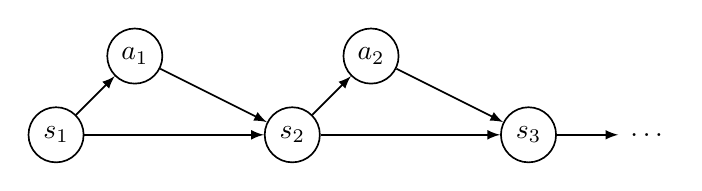
\begin{tikzpicture}[-latex ,auto ,node distance =1 cm and 1cm ,
      on grid , inner sep=0pt, minimum size=7mm,
      semithick, state/.style={circle, draw}]
      % s1, a1, s2;
      \node[state](s_1) at(0,0) {$s_1$};
      \node[state](a_1) at(1,1) {$a_1$};                                                                                                       
      \path (s_1) edge (a_1);
      \node[state](s_2) at(3,0) {$s_2$};
      \path (s_1) edge (s_2);
      \path (a_1) edge (s_2);
      % s2, a2, s3
      \node[state] (a_2) at(4,1) {$a_2$};
      \path (s_2) edge (a_2);
      \node[state] (s_3) at(6,0){$s_3$};
      \path (s_2) edge (s_3);
      \path (a_2) edge (s_3);
      % dots;
      \node (dots) at(7.5,0) {$\ldots$};
      \path (s_3) edge (dots);
  \end{tikzpicture}
  \caption{\label{fig:MDP} Graph of MDP with Markovian states.}
\end{figure}

As mentioned earlier with the robot example, we can have our agent 
not observe the Markovian state, and instead receive an observation, 
$o_t$, from its sensors. This observation is associated with 
an emission operator $\mathcal{E}$, that defines a (possibly stochastic) 
mapping from the state space, $\mathcal{S}$, to the observation 
space, $\mathcal{O}$. This induces a Partially Observed MDP (POMDP) 
whose graphical model is presented in Figure \ref{fig:POMDP}. The 
POMDP is defined by the tuple ($\mathcal{S}$, $\mathcal{A}$, 
$\mathcal{O}$, $\mathcal{P}$, $\mathcal{E}$, $r(\cdot)$, $\gamma$), 
where $\mathcal{O}$ and $\mathcal{E}$ are the observation space and 
the emission operator respectively and everything else in the tuple 
is the same as for the MDP case. It is important to note that the 
reward function is still dependent on the states, and not the observations 
since it specifies the goal and is external to the agent. Intuitively, 
the environment is oblivious to the sensory limitations of the agent 
and only bases its reward signal on the current configuration/state and 
the action that is selected by the agent.

As we 
can read off of the pgm in Figure \ref{fig:POMDP}, we see that given 
$s_t$ and $a_t$, $s_{t+1}$ is still independent of 
$o_{1:t}$, $s_{1:t-1}$ and $a_{1:t-1}$ by D-separation.
The observations, however, are not Markovian in general 
since $o_j$ for $j<t$ 
can influence $o_{t+1}$ even if $o_t$ and $a_t$ are known (again by 
D-separation).

\begin{figure}[H]
  \centering
  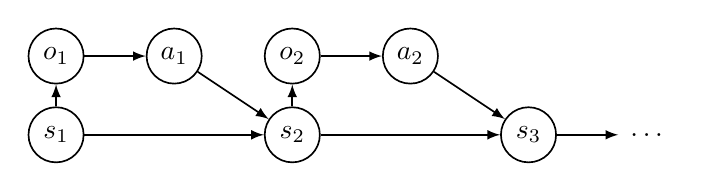
\begin{tikzpicture}[-latex ,auto ,node distance =1 cm and 1cm ,
      on grid , inner sep=0pt, minimum size=7mm,
      semithick, state/.style={circle, draw}]
      % s1, o1, a1, s2;
      \node[state](s_1) at(0,0) {$s_1$};
      \node[state](o_1) at (0, 1){$o_1$};
      \path (s_1) edge (o_1);
      \node[state](a_1) at(1.5,1) {$a_1$};
      \path (o_1) edge (a_1);
      \node[state](s_2) at(3,0) {$s_2$};
      \path (s_1) edge (s_2);
      \path (a_1) edge (s_2);
      % s2, o2, a2, s3
      \node[state](o_2) at (3,1) {$o_2$};
      \path (s_2) edge (o_2);
      \node[state] (a_2) at(4.5,1) {$a_2$};
      \path (o_2) edge (a_2);
      \node[state] (s_3) at(6,0){$s_3$};
      \path (s_2) edge (s_3);
      \path (a_2) edge (s_3);
      % dots;
      \node (dots) at(7.5,0) {$\ldots$};
      \path (s_3) edge (dots);
  \end{tikzpicture}
  \caption{\label{fig:POMDP} Graph of POMDP, $s_t$ is the Markovian 
  state, $o_t$ is the observation of the agent.}
\end{figure}

The associated factorisation based on the pgm in 
Figure \ref{fig:POMDP} is:
\begin{equation}
  p^{\pi}(\tau)=p(s_1)\prod_{t=1}^T p(o_t|s_t)\pi(a_t|o_t)p(s_{t+1}|s_t, a_t).
\end{equation}
We see that in the POMDP setting, the agent makes decisions based 
on the observation and not the Markovian state. Depending on how 
informative the observation is, it may be difficult to construct 
a well-performing policy. Additionally, due to the non-Markovian 
nature of the observations, it is common to track and process old 
observations in order to form the agent state. Intuitively, one 
would expect the influence of observations from a long time ago 
to decay, so it might be useful to have a moving window over the 
collected experience.

In cases where we have deterministic transitions from state and action 
to the next state (and similarly from state to observation), 
$p(s_{t+1}|s_t, a_t)=\delta(s_{t+1},f(s_t, a_t))$, where 
$\delta(\cdot)$ denotes the delta distribution (placing all 
probability mass on $f(s_t, a_t)$) and 
$f: \mathcal{S}\times\mathcal{A}\rightarrow \mathcal{S}$ is some deterministic 
transition function (similarly $g:\mathcal{S}\rightarrow \mathcal{O}$ 
can be the sensor mapping the state to the observation).

%%%%%%%%%%%%%%%%%%%%%%%%%%%%%%%%%%%%%%%%%%%%%%%%%
% SECTION - FORMULATING EPISODIC AND CONTINUAL SETTING REWARD;
\subsection{Formulating objective functions}\label{sec:RLGoalMaths}
In Section \ref{sec:RLGoal} we explained the goal of RL in words. 
In this section we will give a more formal mathematical definition. 
To that end we will first define the finite/episodic case objective, 
and then define the continual setting objective.

First, recall the Monte Carlo return Equation \ref{eq:MCReturn}. The episodic 
objective is to find a behaviour/policy, $\pi(\cdot)$, that maximises 
the expected Monte Carlo return over the distribution of finite 
trajectories, induced by the policy. 
This is summarised by Equation \ref{eq:ep_objective}.
\begin{align}
  \label{eq:ep_objective}
  \pi^*&=\arg \max_{\pi}\; \mathbb{E}_{\tau\sim p^{\pi}(\tau)}[G_0(\tau)]\notag\\
  &=\arg \max_{\pi}\; \mathbb{E}_{\tau\sim p^{\pi}(\tau)}\left[\sum_{t=1}^{len(\tau)}\gamma^{t-1}r(a_{t}, s_{t})\right].
\end{align}
In Equation \ref{eq:ep_objective}, $len(\tau)$ denotes the length of the episode.

Before we tackle the continual setting, observe that the MDP in 
Figure \ref{fig:MDP} can be seen as a Markov chain where we define 
the new state $z_t:=(s_t, a_t)$. Based on this formulation we also 
get a new transition operator 
$p(a_{t+1},s_{t+1}|a_t,s_t)=\pi(a_{t+1}|s_{t+1})p(s_{t+1}|a_t,s_t)$ and 
the corresponding pgm can be observed in Figure \ref{fig:MCz}.

\begin{figure}[H]
  \centering
  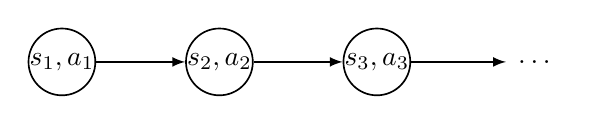
\begin{tikzpicture}[-latex ,auto ,node distance =1 cm and 1cm ,
      on grid , inner sep=0pt, minimum size=7mm,
      semithick, state/.style={circle, draw}]
      % s1, a1, s2;
      \node[state](z_1) at(0,0) {$s_1,a_1$};
      \node[state](z_2) at(2,0) {$s_2, a_2$};
      \path (z_1) edge (z_2);
      \node[state](z_3) at(4,0) {$s_3, a_3$};
      \path (z_2) edge (z_3);
      \node (dots) at(6,0) {$\ldots$};
      \path (z_3) edge (dots);
  \end{tikzpicture}
  \caption{\label{fig:MCz} Markov chain induced by MDP.}
\end{figure}

It can be shown that if the Markov chain is aperiodic and if there 
is a path to all possible tuples $(s_t, a_t)$ from any other tuple 
$(s_j, a_j)$, then an equilibrium distribution exists, which 
tells us the long-term probability of visiting a state-action tuple 
$\mu(s_t, a_t)$.

Observe that we could also rewrite the episodic definition as:
\begin{align}
  \label{eq:cont_objective}
  \pi^*&=\arg \max_{\pi}\; \mathbb{E}_{\tau\sim p^{\pi}(\tau)}[G_0(\tau)]\notag\\
  &=\arg \max_{\pi}\; \mathbb{E}_{\tau\sim p^{\pi}(\tau)}\left[\sum_{t=1}^{len(\tau)}\gamma^{t-1}r(a_{t}, s_{t})\right]\\
  &=\arg \max_{\pi}\; \sum_{t=1}^{maxlen(\tau)}\mathbb{E}_{s_{t}, a_{t}\sim p^{\pi}(s_{t}, a_{t})}[r(s_t, a_t)\gamma^{t-1}]\\
  &=\arg \max_{\pi}\; \frac{1}{maxlen(\tau)}\sum_{t=1}^{maxlen(\tau)}\mathbb{E}_{s_{t}, a_{t}\sim p^{\pi}(s_{t}, a_{t})}[r(s_{t}, a_{t})\gamma^{t-1}],
\end{align}
where $maxlen(\tau)$ is the maximum length of a trajectory possible under $\pi$. 
In the continual setting, $maxlen(\tau)\rightarrow\infty$, and provided the 
equilibrium distribution for the Markov Chain in Figure 
\ref{fig:MCz} exists, 
after some time (burn-in), $p^{\pi}\rightarrow \mu^{\pi}$. Intuitively,
 due to the division by $maxlen(\tau)$, 
the first finite number of steps from $p^{\pi}$ 
will be negligable and only the steps sampled according to the equilibrium, 
$\mu^{\pi}$ will persist. This intuition, helps us arrive at the 
continual objective known as expected long-term reward:
\begin{equation}\label{eq:continualObjective}
  \arg \max_{\pi}\; {E}_{s, a\sim \mu^{\pi}(s, a)}[r(s, a)],
\end{equation}
where $\mu^{\pi}$ is the limiting distribution of the Markov chain 
induced by $\pi$ as seen in Figure \ref{fig:MCz}.



%%%%%%%%%%%%%%%%%%%%%%%%%%%%%%%%%%%%%%%%%%%%%%%%%%%%%%%%%%
% NEW SECTION - VALUE FUNCS;
\subsection{Value functions}\label{sec:valueFuncs}
A key quantity in our application and of much of modern Reinforcement Learning 
are the value functions. These quantities aim to estimate the 
expected future return, given the current state or state-action pair. 
We shall derive those quantities from the RL objective functions 
defined in the previous section.

Starting from the episodic objective Equation \ref{eq:ep_objective},
\begin{align}\label{eq:valFuncDef}
  \mathbb{E}_{\tau\sim p^{\pi}(\tau)}\left[\sum_{t=1}^{len(\tau)}r(s_t, a_t)\gamma^{t-1}\right]
  &=\mathbb{E}_{s_1\sim p(s_1)}\left[\mathbb{E}_{\tau\sim p^{\pi}(\tau|s_1)}\left[\sum_{t=1}^{len(\tau)}r(s_t, a_t)\gamma^{t-1}|s_1\right]\right]\notag\\
  &=\mathbb{E}_{s_1\sim p(s_1)}\left[
      \mathbb{E}_{a_1\sim \pi(\cdot|s_1)}\left[
          r(s_1, a_1) + 
          \mathbb{E}_{\tau\sim p^{\pi}(\tau|s_1,a_1)}\left[\sum_{t=2}^{len(\tau)}r(s_t, a_t)\gamma^{t-1}\right]|s_1,a_1
        \right]
    \right]\notag\\
  &=:\mathbb{E}_{s_1\sim p(s_1)}\left[
      \mathbb{E}_{a_1\sim \pi(\cdot|s_1)}\left[Q^{\pi}(s_1,a_1)\right]
      \right]\notag\\
      &=:\mathbb{E}_{s_1\sim p(s_1)}\left[
        V^{\pi}(s_1)
      \right],
\end{align}
where $Q^{\pi}(s_1,a_1):=\mathbb{E}[G_0(\tau)|s_1, a_1, \pi]$ is the state-action value function,  
sometimes referred to as the Q-function, and $V^{\pi}:=\mathbb{E}_{a_1\sim\pi(\cdot)}[Q^{\pi}(s_1, a_1)|s_1]$ is the state-value 
function.

In Equation \ref{eq:valFuncDef} we already used a form of the Bellman expectation/prediction 
equation:
\begin{align}\label{eq:bellmanv}
  V^{\pi}(s)&=\mathbb{E}_{a\sim \pi(\cdot|s)}[Q^{\pi}(s, a)|s]\notag\\
  &=\mathbb{E}_{a\sim \pi(\cdot|s)}\left[r(s, a) + \gamma \sum_{s'\in \mathcal{S}}p(s'|s,a)V^{\pi}(s')|s\right].
\end{align}

The same for the Q-function is given by Equation \ref{eq:bellmanq}.
\begin{align}\label{eq:bellmanq}
  Q^{\pi}(s, a)&=r(s, a) + \gamma \sum_{s'\in \mathcal{S}}p(s'|s, a)V^{\pi}(s')\notag\\
  &= r(s,a) + \gamma \sum_{s'\in \mathcal{S}}p(s'|s, a)\sum_{a'\in \mathcal{A}}\pi(a'|s')Q^{\pi}(s', a').
\end{align}

The other pair of Bellman equations are known as the Bellman optimality 
equations and enforce a consistency criterion for optimal policies. 
\begin{align}\label{eq:bellmanOptV}
  V^{\pi^*}(s)&=\max_{a\in \mathcal{A}}\; \left[r(s, a) + \gamma \sum_{s'\in \mathcal{S}}p(s'|s,a)V^{\pi}(s')|s\right]\notag\\
  &=\max_{a\in \mathcal{A}}\;Q^{\pi^*}(s, a).
\end{align}

\begin{align}\label{eq:bellmanOptQ}
  Q^{\pi^*}(s,a)&=r(s,a) + \gamma \sum_{s'\in \mathcal{S}}p(s'|s, a)\max_{a'\in \mathcal{A}}\;Q^{\pi*}(s', a').
\end{align}

It can be shown that there always exists at least one optimal 
policy \citep{Sutton1998}, and the Bellman optimality Equations 
in \ref{eq:bellmanOptV} and \ref{eq:bellmanOptQ} can be viewed 
as consistency equations for an optimal policy $\pi^*$.

% SECTION - improving the policy;
\subsection{Policy iteration}
Based on the Value functions, $Q^{\pi}$ and $V^{\pi}$ introduced in the 
previous section, there exists a powerful paradigm that allows 
us to arrive at an optimal policy. This paradim is called Generalised 
Policy Iteration.

Given a policy one might be interested in understanding how good 
it is - evalueate it. Another question, given a current policy, 
might be whether we can improve it. In the tabular case, where 
we can enumarate all state-action pairs, it can be shown that 
for $\gamma\in[0, 1)$, the updates given in Equation 
\ref{eq:policyEval} correspond to operators 
leading to a convergent sequence, whose stationary point is the 
value of the policy $\pi$.
\begin{align}\label{eq:policyEval}
  v_{k+1}(s_t) &\gets \mathbb{E}[r_{t+1} + \gamma v_k(s_{t+1})|s_t]\notag\\
  q_{k+1}(s_t, a_t)&\gets r(s_t, a_t) 
  + \gamma\mathbb{E}[q_{k}(s_{t+1}, a_{t+1})|s_t,a_t].
\end{align}

We can iterate the Equations in \ref{eq:policyEval} until $v_{k+1}(s)=v_k(s)$ 
$\forall s\in \mathcal{S}$ at which point we get $v_k\approx v^{\pi}$ 
(and similarly for $q$).


For the policy improvement step, it can be shown \citep{Sutton1998} 
that after the 
policy evaluation converges, updating the policy 
to be greedy with respect to the action value $q^{\pi}$ of the 
current policy, improves the policy.
\begin{equation}\label{eq:policyImp}
  \pi'(s)=\arg \max_a q^{\pi}(s, a).
\end{equation}

Together, the Equations for policy evaluation \ref{eq:policyEval} 
and policy improvement \ref{eq:policyImp} 
can be iterated one after another until we reach an optimal policy 
given an MDP.

It is worth noting, that instead of waiting for policy evaluation 
to converge, we can instead do just one sweep 
of updates (single iteration) and then immediately do a policy 
improvement step. This procedure is known as value iteration and 
can also be shown to converge to the value functions of an 
optimal policy given an MDP. The equations for value iteration 
are shown in \ref{eq:valueIter}
\begin{align}\label{eq:valueIter}
  v_{k+1}(s_t)&\gets\max_a \left[r(s_t, a) 
  + \gamma \sum_{s'\in\mathcal{S}}p(s'|s_t, a)v_{k}(s')\right]\notag\\
  q_{k+1}(s_t, a_t)&\gets r(s_t, a_t) 
  + \gamma \sum_{s'\in\mathcal{S}}p(s'|s_t, a_t)\max_a\; q_{k}(s', a).
\end{align}


%%%%%%%%%%%%%%%%%%%%%%%%%%%
% NEW SECTION - Q-learning;
\subsection{Q-learning}\label{sec:Qlearning}
In this section we use Q-learning \citep{QlearningWatkins1992} 
as a motivating example 
for single-step off-policy methods. These are methods 
that aim to evaluate a target policy, $\pi$, while following 
a different behaviour policy, $\mu$. This will be relevant when 
we describe the algorithm \citep{SAC2} 
used in the inner loop of our IRL routine.

The simplest way to understand Q-learning, is perhaps by 
first introducing an on-line variant called SARSA \citep{SARSA}. 
SARSA is an algorithm that samples the policy evaluation update 
for the Q-function as given in Equation \ref{eq:policyEval}.
The sampling is done based on the current policy/behaviour and can 
be motivated by gradient descent on the Mean Squared Error of 
the true Q-function, $Q^{\pi}$, and our current estimate $Q_{k}$.
Intuitively, taking a gradient with respect to $Q_{k}$ we get the 
expression in Equation \ref{eq:sarsaGrad}.
\begin{align}\label{eq:sarsaGrad}
  \frac{\partial}{\partial Q_{k}}(Q^{\pi}(s_t, a_t) - Q_{k}(s_t, a_t))^2&=-2(Q^{\pi}(s_t, a_t) - Q_{k}(s_t,a_t)).
\end{align}

Since we do not know the true $Q^{\pi}$ (otherwise we would be done) 
we receive a reward, $r_{t+1}$, and the next state $s_{t+1}$ 
based on taking action $a_t$ at state $s_t$, then sample the next 
action, $a_{t+1}$, according to the current policy and instead of the 
true Q-function, we use our estimate $Q_{k}(s_{t+1}, a_{t+1})$ to evaluate 
the next state-action pair. This process gives the update in 
Equation \ref{eq:sarsa}.
The technique for using $Q_{k}(s_{t+1}, a_{t+1})$ instead 
of $Q^{\pi}(s_{t+1}, a_{t+1})$ is known as bootstrapping and needs to be 
handled with care since it is not 
necessarily a good estimate of $Q^{\pi}(s_{t+1}, a_{t+1})$ (it is biased). 
To this end, take note of the learning rate, $\alpha$ in Equation 
\ref{eq:sarsa} which is there to account for the noise introduced 
by bootstrapping.

Note that we did not require access to the model, $\mathcal{P}$, at 
any point. Because of this, SARSA is classified as a model-free method.

\begin{equation}\label{eq:sarsa}
  Q_{k+1}(s_t, a_t) = Q_{k}(s_t, a_t) + \alpha (r_{t+1} + \gamma Q_{k}(s_{t+1}, a_{t+1}) - Q_{k}(s_t, a_t)).
\end{equation}

% In Equation \ref{eq:sarsa}, first we interact with the environment 
% by proposing $a_t$, sampled by the current policy, then the environment 
% gives us the reward $r$ as feedback and transitions to the next state 
% $s_{t+1}$. At this point we once again sample an action $a_{t+1}$ 
% from the current policy and update in a gradient descent on the 
% Q-value fashion, towards the reward plus the discounted Q-value for 
% the next state action pair, $(s_{t+1},\; a_{t+1})$.

While SARSA evaluates the current policy $\pi$, Q-learning aims 
to evaluate the greedy policy given the current estimate $Q_{k}$, 
while following another policy, $\mu$, known as the behaviour. 
This is why Q-learning is an off-policy method.

The associated update (for tabular Q-learning) is given in Equation 
\ref{eq:qlearning}
\begin{equation}\label{eq:qlearning}
  Q_{k+1}(s_t, a_t) = Q_{k}(s_t, a_t) + \alpha \left(r_{t+1} + \gamma \max_{a'\in\mathcal{A}}\;Q_{k}(s_{t+1}, a') - Q_{k}(s_t, a_t)\right).
\end{equation}

The reader may have noticed that the update for Q-learning is like 
a sampled version of the value iteration Equation \ref{eq:valueIter} 
for the Q-function. Both SARSA and Q-learning can be shown to 
converge given appropriately decaying learning rates $\alpha$ 
that satisfy the Robbins-Monro conditions given in Equation 
\ref{eq:RobbinsMonro} and a behaviour, $\mu$ that explores 
sufficiently often (needed for Q-learning).

\begin{align}\label{eq:RobbinsMonro}
  \sum_{k=0}^\infty \alpha_k&\rightarrow \infty\notag\\
  \sum_{k=0}^\infty \alpha_k^2&< \infty.
\end{align}

%%%%%%%%%%%%%%%%%%%%%%%%%%%%%%%%%%%%%%%5
% NEW SECTION;
\subsection{Policy Gradients}\label{sec:PolicyGrads}
In the previous sections we have focused on ways to estimate 
value functions, which we can then use to derive a policy implicitly. 

In this section we introduce methods from 
the policy-based RL family, where we explicitly 
parameterise a policy function 
$\pi_\theta$ and aim to estimate its parameters. This is perhaps 
the most direct-looking way to achieve the goal of RL as defined 
in Section \ref{sec:RLGoal}.

Before we begin, it is worth inspecting the pgm of the MDP
in Figure \ref{fig:MDPRew}, 
this time having included the rewards. Note how the reward 
at time $t$ does not depend on future actions and/or states 
given the state and action at time $t-1$.
\begin{figure}[H]
  \centering
  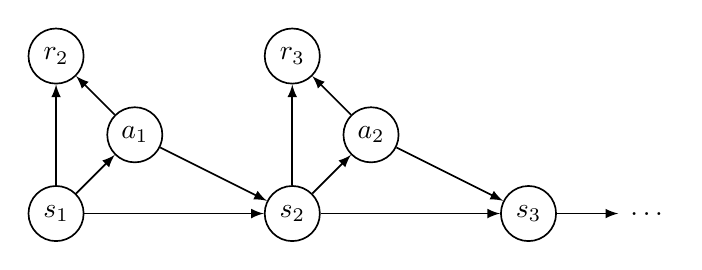
\begin{tikzpicture}[-latex ,auto ,node distance =1 cm and 1cm ,
      on grid , inner sep=0pt, minimum size=7mm,
      semithick, state/.style={circle, draw}]
      % s1, a1, s2;
      \node[state](s_1) at(0,0) {$s_1$};
      \node[state](a_1) at(1,1) {$a_1$};                                                                                                       
      \path (s_1) edge (a_1);
      \node[state](r_2) at(0, 2) {$r_2$};
      \node[state](s_2) at(3,0) {$s_2$};
      \path (s_1) edge (s_2);
      \path (a_1) edge (s_2);
      \path (s_1) edge (r_2);
      \path (a_1) edge (r_2);
      % s2, a2, s3
      \node[state] (a_2) at(4,1) {$a_2$};
      \path (s_2) edge (a_2);
      \node[state] (r_3) at(3, 2) {$r_3$};
      \node[state] (s_3) at(6,0){$s_3$};
      \path (s_2) edge (s_3);
      \path (a_2) edge (s_3);
      \path (s_2) edge (r_3);
      \path (a_2) edge (r_3);
      % dots;
      \node (dots) at(7.5,0) {$\ldots$};
      \path (s_3) edge (dots);
  \end{tikzpicture}
  \caption{\label{fig:MDPRew} Graph of MDP including rewards.}
\end{figure}

We derive Policy Gradients \citep{REINFORCE} 
by starting from the episodic objective as introduced in Section 
\ref{sec:RLGoalMaths}. Due to parameterising our policy 
with parameters, $\theta$, and assuming it is among a 
class of functions who are 
differentiable in $\theta$, we reformulate the episodic 
objective as given in Equation \ref{eq:PGObjective}.

\begin{align}\label{eq:PGObjective}
  J_\theta&:=\mathbb{E}_{\tau\sim p_{\theta}(\tau)}
   \left[
    \sum_{t=1}^{len(\tau)}\gamma^{t-1}r(a_t, s_t)\right]\notag\\ 
  \theta^*&=\arg \max_{\theta}J_\theta.
\end{align}

The gradient of this objective with respect to the parameters, $\theta$ 
of the policy is derived in Equation \ref{eq:PGDerive}.
\begin{align}\label{eq:PGDerive}
  \nabla J_\theta&=\nabla\sum_{\tau}p_{\theta}(\tau)\sum_{t=1}^{\text{len}(\tau)}\gamma^{t-1}r(s_t, a_t)\notag\\
  &=\sum_{\tau}\nabla p_{\theta}(\tau)\sum_{t=1}^{\text{len}(\tau)}\gamma^{t-1}r(s_t, a_t)\notag\\
  &=\sum_{\tau}p_{\theta}(\tau)\nabla \log p_\theta(\tau)\sum_{t=1}^{\text{len}(\tau)}\gamma^{t-1}r(s_t, a_t)\notag\\
  &=\sum_{\tau}p_{\theta}(\tau)\left(
    \sum_{t=1}^{\text{len}(\tau)}\nabla \log \pi_\theta(a_t|s_t)
  \right)\sum_{k=1}^{\text{len}(\tau)}\gamma^{k-1}r(s_k, a_k)\notag\\
  &=\sum_{\tau}p_\theta(\tau)\sum_{t=1}^{\text{len}(\tau)}\nabla \log \pi_\theta(a_t|s_t)
  \left(
    \sum_{k=1}^{t-1}\gamma^{k-1}r(s_k, a_k)
    + \sum_{k=t}^{\text{len}(\tau)}\gamma^{k-1}r(s_k, a_k)
  \right)\notag\\
  &=\sum_{\tau}p_\theta(\tau)\sum_{t=1}^{\text{len}(\tau)}\nabla \log \pi_\theta(a_t|s_t)
  \left(
    \sum_{k=t}^{\text{len}(\tau)}\gamma^{t-1}r(s_k, a_k)
  \right)\notag\\
  &=\sum_{\tau}p_\theta(\tau)\sum_{t=1}^{\text{len}(\tau)}\nabla \log \pi_\theta(a_t|s_t)
  \gamma^{t-1}\left(
    \sum_{k=t}^{\text{len}(\tau)}\gamma^{k-t}r(s_k, a_k)
  \right)\notag\\
  &=\sum_{\tau}p_\theta(\tau)\sum_{t=1}^{\text{len}(\tau)}\nabla \log \pi_\theta(a_t|s_t)
  \gamma^{t-1}G_t(\tau_{t:})\notag\\
  &=\mathbb{E}_{\tau\sim p_\theta(\tau)}\left[\sum_{t=1}^{\text{len}(\tau)}\nabla \log \pi_\theta(a_t|s_t)
  \gamma^{t-1}G_t(\tau_{t:})\right]\notag\\
  &=\mathbb{E}_{\tau\sim p_\theta(\tau)}\left[\sum_{t=1}^{\text{len}(\tau)}\nabla \log \pi_\theta(a_t|s_t)
  \gamma^{t-1}Q^{\pi}(s_t, a_t)\right].
\end{align}

While deriving Equation \ref{eq:PGDerive} we have used the 
fact in Equation \ref{eq:dropPrevRews}.

\begin{align}\label{eq:dropPrevRews}
  \sum_{\tau}p_\theta(\tau)\nabla \log \pi_\theta(a_t|s_t)
  \left(
    \sum_{k=1}^{t-1}\gamma^{k-1}r(s_k, a_k)
  \right)\notag\\
  &=\sum_{\tau_{:t}}p_\theta(\tau_{:t})\left(
    \sum_{k=1}^{t-1}\gamma^{k-1}r(s_k, a_k)
  \right)\sum_{a_t\in\mathcal{A}}\pi_\theta(a_t|s_t)
  \nabla \log \pi(a_t|s_t)\sum_{\tau_{t+1:}}p_\theta(\tau_{t+1:})\notag\\
  &=\sum_{\tau_{:t}}p_\theta(\tau_{:t})\left(
    \sum_{k=1}^{t-1}\gamma^{k-1}r(s_k, a_k)
  \right)\sum_{a_t\in\mathcal{A}}\pi_\theta(a_t|s_t)
  \nabla \log \pi(a_t|s_t)\notag\\
  &=\sum_{\tau_{:t}}p_\theta(\tau_{:t})\left(
    \sum_{k=1}^{t-1}\gamma^{k-1}r(s_k, a_k)
  \right)\sum_{a_t\in\mathcal{A}}\pi_\theta(a_t|s_t)\frac{\nabla\pi(a_t|s_t)}{\pi_\theta(a_t|s_t)}\notag\\
  &=\sum_{\tau_{:t}}p_\theta(\tau_{:t})\left(
    \sum_{k=1}^{t-1}\gamma^{k-1}r(s_k, a_k)
  \right)\nabla\sum_{a_t\in\mathcal{A}}\pi_\theta(a_t|s_t)\notag\\
  &=\sum_{\tau_{:t}}p_\theta(\tau_{:t})\left(
    \sum_{k=1}^{t-1}\gamma^{k-1}r(s_k, a_k)
  \right)\times 0\notag\\
  &=0.
\end{align}

Where in the above we used the short-hand notation:
\begin{align*}
  \sum_{\tau_{:t}}p_\theta(\tau_{:t})&=\sum_{s_1,a_1,\ldots,s_t}p(s_1)\prod_{k=1}^{t-1}\pi_\theta(a_k|s_k)p(s_{k+1}|s_k,a_k),\notag\\
  \sum_{\tau_{t+1:}}p_\theta(\tau_{t+1:})&=\sum_{s_{t+1}, a_{t+1},\ldots,s_{\text{len}(\tau)}}p(s_{t+1}|s_t,a_t)\prod_{k=t+1}^{\text{len}(\tau)-1}\pi(a_k|s_k)p(s_{k+1}|s_k,a_k).
\end{align*}

Taking a closer look at Equation \ref{eq:PGDerive}, we see that 
if we sample it, we get Equation \ref{eq:sampledPG}.
\begin{equation}\label{eq:sampledPG}
  \sum_{n=1}^N
    \sum_{t=1}^{\text{len}(\tau^{(n)})}\nabla \log \pi_\theta(a_t^{(n)}|s_t^{(n)})
  \gamma^{t-1}G_t(\tau_{t:}^{(n)}).
\end{equation}

This is very similar to maximum likelihood estimation of $\theta$ 
given trajectories sampled according to $p_\theta$, however, 
also weighted by a discounted return $\gamma^{t-1}G_t(\tau_{t:}^{(n)})$.
Intuitively, we wish to maximise the likelihood of trajectories 
that resulted in greater returns.

\subsection{Actor-Critics}
In Section \ref{sec:PolicyGrads} we derived the policy gradient 
update rule and gave an intuitive relation to maximum likelihood 
where we wish to increase the likelihood of episodes resulting 
in greater returns. This makes the policy gradients dependent of 
the form of the returns. Suppose the high returns are zeros and 
the low returns are negative. If the high returns are zeros, then 
the update associated with them will vanish. This makes the policy 
gradients dependent on the type of reward function of the environment 
and can cause policy gradients to be very noisy in finite samples.

Actor Critics \citep{Tsitsiklis} are a way to aleviate this issue 
by introducing a baseline function, to which the returns are compared.
Returns who score higher than the baseline are associated with 
beneficial behaviour and we wish to increase the likelihood 
of actions leading to such behaviour/returns.

To make this concrete, consider the baseline $b(s_t)$, that depends 
on $s_t$.

\begin{theorem}\label{thm:baselineThm}
  \begin{equation*}
    \mathbb{E}_{\tau\sim p_\theta(\tau)}\left[\nabla \log \pi_\theta(a_t|s_t)
    b(s_t)\right]=0.  
  \end{equation*}
\end{theorem}

\begin{proof}
  \begin{align}
    \mathbb{E}_{\tau\sim p_\theta(\tau)}\left[\nabla \log \pi_\theta(a_t|s_t)
    b(s_t)\right]&= \sum_{\tau}p_\theta(\tau)\nabla \log\pi_\theta(a_t|s_t)b(s_t)\notag\\
    &=\sum_{\tau_{:t}}p_\theta(\tau_{:t})b(s_t)\sum_{a_t\in\mathcal{A}}\pi_\theta(a_t|s_t)\nabla \log\pi_\theta(a_t|s_t) \sum_{\tau_{t+1:}}p_\theta(\tau_{t+1:})\notag\\
    &=\sum_{\tau_{:t}}p_\theta(\tau_{:t})b(s_t)\sum_{a_t\in\mathcal{A}}\pi_\theta(a_t|s_t)\nabla \log\pi_\theta(a_t|s_t)\notag\\
    &=\sum_{\tau_{:t}}p_\theta(\tau_{:t})b(s_t)\times 0\notag\\
    &=0,
  \end{align}
  where, similarly to in the policy gradient derivation, we used the fact that 
  \begin{equation*}
    \sum_{a_t\in\mathcal{A}}\pi_\theta(a_t|s_t)\nabla \log\pi_\theta(a_t|s_t)=0. 
  \end{equation*}
\end{proof}

Based on Theorem \ref{thm:baselineThm} we have that:
\begin{theorem}\label{thm:unbiasedBaseline}
  Given a baseline, $b(s_t)$, that does not depend on the actions,\\
  $\mathbb{E}_{\tau\sim p_\theta(\tau)}\left[\sum_{t=1}^{\text{len}(\tau)}\nabla \log \pi_\theta(a_t|s_t)
  \gamma^{t-1}\left(Q^{\pi}(s_t, a_t)-b(s_t)\right)\right]$ is unbiased with respect 
  to the policy gradient update in Equation \ref{eq:PGDerive}.
\end{theorem}
Due to Theorem \ref{thm:baselineThm}, we can pick any function 
$b(\cdot)$ that does not depend on the actions as a baseline and 
get an unbiased policy gradient update. In the case of Actor-Critics, 
$b(s_t)=V^{\pi}(s_t)$, or an approximation thereof, $V_{\phi}$.

The Actor-Critic update is then given in Equation \ref{eq:ActorCritic}.
\begin{equation}\label{eq:ActorCritic}
  \mathbb{E}_{\tau\sim p_\theta(\tau)}\left[\sum_{t=1}^{\text{len}(\tau)}\nabla \log \pi_\theta(a_t|s_t)
  \gamma^{t-1}\left(Q^{\pi}(s_t, a_t)-V^{\pi}(s_t)\right)\right].
\end{equation}

The term $Q^{\pi}(s_t,a_t)-V^{\pi}(s_t)$ is sometimes called the 
advantage due to taking action $a_t$ at state $s_t$. This is 
due to the Bellman Expectation equation for the state-value function 
as given in Equation \ref{eq:bellmanv}. Since $V^{\pi}$ is the 
expected Q-function, integrating over the actions, there are 
actions for which the Q-function is greater than or equal to the 
state-value function. Such actions are advantageous, since they are 
likely to lead us to trajectories that yield high returns (since the 
Q-function is itself the expected future return given start at 
the relevant state and action). The Actor-Critic aims to 
increase the likelihood of advantageous actions, therefore.

In practice, $V^{\pi}$ is approximated by e.g., a parameterised 
state-value function $V_\psi$, which is learned by some policy 
evaluation method. Such methods can be as simple as just 
substituting the Q-function for the state-value function 
in the Equation for SARSA \ref{eq:sarsa}, which results in 
a method called TD(0) \citep{SuttonTD}. 
The Q-function, $Q^{\pi}$ is often also approximated 
either by the relevant Monte Carlo return as given in Equation 
\ref{eq:MCReturn} or by bootstrapping as in the 
case of SARSA.

\subsection{Maximum Entropy Reinforcement Learning}\label{sec:MaxEntRL}
Maximum Entropy Reinforcement Learning (MaxEntRL) is most commonly 
motivated by observing the behaviour of biological systems, assuming 
they are rational agents and that they act the way they do in order to achieve 
a certain goal. The crucial point here is that although all 
demonstrations are assumed to achieve the goal of the agent, 
they are allowed to deviate from one-another in ways that 
do not impact their successful outcome. That being said, 
some demonstrations may be more desirable than others, e.g., 
because they make fewer unnecessary steps to achieve the goal.

This definition makes 
traditional optimal control theory inappropriate for modelling 
this behaviour and understanding why we observed the different 
paths. This is because, it can be shown that under the objective 
introduced in Section \ref{sec:RLGoalMaths}, given full observability 
(Markov states), there exists an optimal policy that 
is deterministic \citep{Sutton1998}.
This cannot help us explain the variability in the agent's demonstrations,
therefore.

In order to be able to learn a good behaviour, we still 
need to somehow differentiate between demonstrations and tell 
which ones are more desirable to emulate. 
In his paper \cite{Ziebart2008} aims to create an ordering among 
observed demonstrations by weighting the trajectories 
by the exponential of the sum of rewards (the return) along 
the given trajectory. In this way, demonstrations with greater 
returns 
will be exponentialy more desirable than others. A simple illustration 
of the soft-optimal control (SOC) idea is portrayed in Figure \ref{fig:softopt}. 
In this figure, we see the optimal control behaviour, and the 
soft-optimal demonstrations alongside it.


\begin{figure}[H]
  \begin{center}
    \includegraphics[scale=0.5]{optControlVsSoftOpt.png}
  \end{center}
  \caption{\label{fig:softopt}Simple illustration of Optimal Control vs Soft optimal 
  Control. The blue solid line represents the deterministic optimal 
  control to reach from the red ``X'' on the left to the 
  red ``X'' on the right. The remaining lines 
  are noisy perturbations of the intermediate points 
  between the starting and ending ``X'' - demonstrating 
  soft optimality.}
\end{figure}

A very illustrative way to understand soft-optimal control (SOC) 
is provided in \cite{LevineRLasInf}, where the associated 
pgm is a Directed Acyclic Graph (DAG) such as the one 
seen in Figure \ref{fig:SOCGraph}.

\begin{figure}[H]
  \centering
  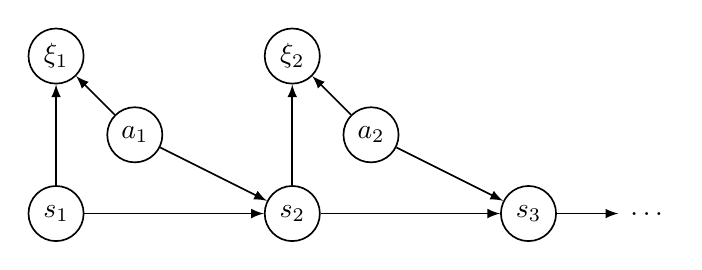
\begin{tikzpicture}[-latex ,auto ,node distance =1 cm and 1cm ,
      on grid , inner sep=0pt, minimum size=7mm,
      semithick, state/.style={circle, draw}]
      % s1, a1, s2;
      \node[state](s_1) at(0,0) {$s_1$};
      \node[state](a_1) at(1,1) {$a_1$};                                                                                                       
      % \path (s_1) edge (a_1);
      \node[state](xi_1) at(0, 2) {$\xi_1$};
      \node[state](s_2) at(3,0) {$s_2$};
      \path (s_1) edge (s_2);
      \path (a_1) edge (s_2);
      \path (s_1) edge (xi_1);
      \path (a_1) edge (xi_1);
      % s2, a2, s3
      \node[state] (a_2) at(4,1) {$a_2$};
      % \path (s_2) edge (a_2);
      \node[state] (xi_2) at(3, 2) {$\xi_2$};
      \node[state] (s_3) at(6,0){$s_3$};
      \path (s_2) edge (s_3);
      \path (a_2) edge (s_3);
      \path (s_2) edge (xi_2);
      \path (a_2) edge (xi_2);
      % dots;
      \node (dots) at(7.5,0) {$\ldots$};
      \path (s_3) edge (dots);
  \end{tikzpicture}
  \caption{\label{fig:SOCGraph} Graph of Soft-Optimal model. 
  The $\xi$ variables are binary optimality variables, equal to 
  $1$ with probability equal to $\exp(r(s_t, a_t))$.}
\end{figure}

Outside of the usual RL variables - states and actions - here, 
we also have binary ``optimality'' variables, $\xi_t\sim \text{Ber}(\exp(r(s_t, a_t)))$.
Where $\text{Ber}(\cdot)$ denotes the Bernoulli distribution. 
This means that we require the reward to be non-positive, which 
is easily achieved (in the case of bounded rewards) by subtracting 
the maximum reward.

It is worth noting that 
in \cite{Ziebart2008}, the graph is a Markov Random Field (MRF) 
where the states and actions share a potential function given 
by $\exp(r(s_t, a_t))$. This allows
the rewards to be positive.

We have chosen the formulation in \cite{LevineRLasInf} 
since it allows us to more 
easily convey the motivations behind SOC and later describe the 
algorithm used in the inner loop of the IRL problem \citep{SAC2}.

Based on the model defined by the pgm in Figure \ref{fig:SOCGraph}, 
we wish to estimate the policy of the agent, $p(a_t|s_t, \xi_{1:T}=1)$, 
assuming $\xi_t=1\;\forall t$, 
i.e., that the demonstrations are ``softly'' optimal. 
To this end, we employ the technique of message passing, and perform 
computations very similar to the ones performed in Hidden Markov Models 
(HHM).

Before we proceed with the derivations,
we first define short-hand notation in Equation \ref{eq:messages}, 
where $\beta$ are backward messages and $\alpha$ are forward messages.
\begin{align}\label{eq:messages}
  \beta_t(s_t, a_t)&:=p(\xi_{t:T}=1|s_t, a_t)\notag\\
  \beta_t(s_t)&:=p(\xi_{t:T}=1|s_t)\notag\\
  \alpha_t(s_t)&:=p(s_t, \xi_{1:t-1}=1).
\end{align}

The derivation of the message passing procedure can be seen 
in Equations \ref{eq:SOCQmessage}, \ref{eq:SOCVmessage} and 
\ref{eq:SOCforwardMessage}. Note that for brevity, we will use 
$\xi_{t:T}$ to mean $\xi_{t:T}=1$, i.e., that all optimality variables 
are equal to one.

\begin{align}\label{eq:SOCQmessage}
  \beta_t(s_t, a_t)&:=p(\xi_{t:T}=1|s_t, a_t)\notag\\
  &=p(\xi_t|s_t, a_t)p(\xi_{t+1:T}|s_t, a_t)\notag\\
  &=p(\xi_t|s_t, a_t)\int_{\mathcal{S}}p(\xi_{t+1:T}, s_{t+1}|s_t,a_t)ds_{t+1}\notag\\
  &=p(\xi_t|s_t, a_t)\int_{\mathcal{S}}p(\xi_{t+1:T}|s_{t+1})p(s_{t+1}|s_t,a_t)ds_{t+1}\notag\\
  &=p(\xi_t|s_t, a_t)\mathbb{E}_{s_{t+1}\sim p(s_{t+1}|s_t, a_t)}[\beta_t(s_{t+1})]\notag\\
  &=\exp(r(s_t, a_t))\mathbb{E}_{s_{t+1}\sim p(s_{t+1}|s_t, a_t)}[\beta_t(s_{t+1})].
\end{align}

\begin{align}\label{eq:SOCVmessage}
  \beta_t(s_t)&:=p(\xi_{t:T}|s_t)\notag\\
  &=\int_{\mathcal{A}}p(\xi_{t:T},a_t|s_t)da_t\notag\\
  &=\int_{\mathcal{A}}p(\xi_{t:T}|a_t, s_t)p(a_t|s_t)\notag\\
  &=\mathbb{E}_{a_t\sim p(a_t|s_t)}[\beta_t(s_t, a_t)].
\end{align}

\begin{align}\label{eq:SOCforwardMessage}
  \alpha_t(s_t)&:=p(s_t, \xi_{1:t-1}=1)\notag\\
  &=\int_{\mathcal{S}}\int_{\mathcal{A}}p(s_t, s_{t-1},a_{t-1},\xi_{1:t-1})da_{t-1}ds_{t-1}\notag\\
  &=\int_{\mathcal{S}}\int_{\mathcal{A}}p(s_t|s_{t-1}a_{t-1})p(\xi_{t-1}|s_{t-1},a_{t-1})p(a_{t-1}|s_{t-1})p(s_{t-1}, \xi_{1:t-2})da_{t-1}ds_{t-1}\notag\\
  &=\int_{\mathcal{S}}\int_{\mathcal{A}}p(s_t|s_{t-1}a_{t-1})p(\xi_{t-1}|s_{t-1},a_{t-1})p(a_{t-1}|s_{t-1})\alpha_{t-1}(s_{t-1})da_{t-1}ds_{t-1}.
\end{align}

In the above, $p(a_t|s_t)$ is not to be confused for the policy, 
$p(a_t|s_t, \xi_{1:T}=1)$. The interpretation of $p(a_t|s_t)$ 
is merely as a prior belief about what actions are 
possible given the state. 
Note that $p(a_t|s_t)$ is not conditioned on optimality variables, 
$\xi$, so it makes sense to substitute it for a uniform prior 
(since no particualr behaviour is assumed of the agent). Later 
we will discuss how it is possible to specify a non-trivial prior.


First, let us focus our attention on the backward messages, 
$\beta_t(s_t, a_t)$ and $\beta_t(s_t)$. 
Based on the backward messages we can calculate the policy as 
shown in Equation \ref{eq:policyMessage}.
\begin{align}\label{eq:policyMessage}
  p(a_t|s_t,\xi_{1:T})&=p(a_t|s_t,\xi_{t:T})\notag\\
  &=\frac{p(\xi_{t:T},s_t,a_t)}{p(s_t,\xi_{t:T})}\notag\\
  &=\frac{p(\xi_{t:T}|s_t, a_t)p(a_t|s_t)p(s_t)}{p(\xi_{t:T}|s_t)p(s_t)}\notag\\
  &=\frac{\beta(s_t, a_t)p(a_t|s_t)}{\beta(s_t)}.
\end{align}

Now, let us define some 
suggestive notation based on the backward messages as shown 
in Equation \ref{eq:backMsgsAsVals}.
\begin{align}\label{eq:backMsgsAsVals}
  Q(s_t, a_t)&=\log \beta(s_t, a_t)\notag\\
  V(s_t)&=\log \beta(s_t).
\end{align}

If we think of the backward messages as the exponentiated 
value functions, based on Equations \ref{eq:SOCQmessage} and 
\ref{eq:SOCVmessage}, we see that:
\begin{align}\label{eq:badVals}
  Q(s_t, a_t)&=\log p(\xi_t|s_t, a_t) + \log\mathbb{E}_{s_{t+1}\sim p(s_{t+1}|s_t, a_t)}[\exp (V(s_{t+1}))]\notag\\
  &=r(s_t, a_t) + \log\mathbb{E}_{s_{t+1}\sim p(s_{t+1}|s_t, a_t)}[\exp (V(s_{t+1}))]\notag\\
  V(s_t)&=\log \int_{\mathcal{A}}\exp (Q(s_t, a_t))p(a_t|s_t)da_t.
\end{align}

It turns out that if we wish to give some prior for the actions, 
other than uniform, we can just augment the reward function 
by adding $\log p(a_t|s_t)$ to it and still treat $p(a_t|s_t)$ 
as if it is uniform and ignore it. This is shown in Equation 
\ref{eq:priorMsgs}.
\begin{align}\label{eq:priorMsgs}
  V(s_t)&=\log \int_{\mathcal{A}}\exp (Q(s_t, a_t) + \log p(a_t|s_t))da_t\notag\\
  &=\log \int_{\mathcal{A}}\exp (\hat{Q}(s_t, a_t))da_t.
\end{align}

Ignoring the $p(a_t|s_t)$ term, 
the policy equation becomes just the ratio 
of the two messages as shown in Equation \ref{eq:policyMessageNoPrior}.

\begin{align}\label{eq:policyMessageNoPrior}
  p(a_t|s_t, \xi_{1:T}=1)&=\frac{\beta(s_t, a_t)}{\beta(s_t)}\notag\\
  &=\exp(Q(s_t, a_t) - V(s_t)),
\end{align}
where we have augmented the reward $\hat{r}(s_t, a_t)=r(s_t,a_t) + \log p(a_t|s_t)$.
Observe that the expression for $p(a_t|s_t,\xi_{1:T}=1)$ in Equation 
\ref{eq:policyMessageNoPrior} is an advantage-like function based on 
the current message-based value functions. This form will prove 
important in the later sections.

Turning our attention back to Equation \ref{eq:badVals}, however, 
we observe that the current definition of the Q-function is 
over-optimistic (unless $p(s_{t+1}|s_t,a_t$ is deterministic). 
This is can be shown by Jensen's inequality and 
is displayed in Equation \ref{eq:OverestimatedQ}.

\begin{align}\label{eq:OverestimatedQ}
  Q(s_t,a_t)&=r(s_t, a_t) + \log\mathbb{E}_{s_{t+1}\sim p(s_{t+1}|s_t, a_t)}[\exp (V(s_{t+1}))]\notag\\
  &\ge r(s_t, a_t) + \mathbb{E}_{s_{t+1}\sim p(s_{t+1}|s_t, a_t)}[V(s_{t+1})].
\end{align}

More intuition for why we are overestimating the Q-function 
via this message-passing procedure can be gained by writing 
out the likelihood of a soft-optimal path, $p(\tau|\xi_{1:T}=1)$. 
Observing Equation \ref{eq:changedDynamics}, we see that due to 
assuming soft-optimal trajectories, we have changed the dynamics 
of the MDP from $p(s_{t+1}|s_t, a_t)$ to 
$p(s_{t+1}| s_t,a_t,\xi_{t:T}=1)$.

\begin{align}\label{eq:changedDynamics}
  p(\tau|\xi_{1:T}=1)&=p(s_1|\xi_{1:T}=1)\prod_{t=1}^Tp(a_t|s_t,\xi_{t:T}=1)p(s_{t+1}|s_t, a_t, \xi_{t:T}=1).
\end{align}

Now we need to come up with a way to keep the dynamics of the MDP 
while still being able to compute a policy. 
We can achieve this by Variational Inference. Before we continue, 
we derive a general form for an optimal distribution using 
the Calculus of Variations. This can be seen in Theorem \ref{thm:OptDist}.

\begin{theorem}\label{thm:OptDist}
  The distribution, $q(\cdot)$ that maximises the expression 
  $\int q(x)f(x)dx + \mathcal{H}[q]$, where $\mathcal{H}[q]=-\int q(x)\log q(x)dx$
  is the entropy 
  and $f(x)$ is an integrable function on the domain of $q(x)$, 
  is proportional to $\exp (f(x))$.
\end{theorem}

\begin{proof}
  First we add a Lagrangian term, $\lambda(\int q(x)dx - 1)$ to 
  enforce the constraint that $q(\cdot)$ is a valid probability 
  distribution.
  \begin{align}
    J&:=\int q(x)f(x)dx + \mathcal{H}[q] + \lambda(\int q(x)dx - 1).
  \end{align}
  Now taking a variational derivative with respect to $q(x)$,
  \begin{align}
    \frac{\delta J}{\delta q(x)} &=0\notag\\
    \iff f(x) - \log q(x) - 1 + \lambda &=0\notag\\
    \iff q(x)\propto \exp(f(x)).
  \end{align}
\end{proof}

Now we proceed to approximating the likelihood of the trajectory, 
given that it is optimal using the functional form in Equation 
\ref{eq:ApproxDist}.

\begin{equation}\label{eq:ApproxDist}
  q(\tau)=p(s_1)\prod_{t=1}^Tq_t(a_t|s_t)p(s_{t+1}|s_t,a_t).
\end{equation}

Recall the general equation for the free energy (also known as ELBO) 
used in the EM algorithm, given in Equation \ref{eq:FreeEnergy}.

\begin{align}\label{eq:FreeEnergy}
  \log p(x)&=\log \int p(x,z)dz\notag\\
  &=\log \int q(z)\frac{p(x,z)}{q(z)}dz\notag\\
  &\ge \mathbb{E}_{z\sim q(z)}\left[\log \frac{p(x, z)}{q(z)}\right].
\end{align}

The last line in Equation \ref{eq:FreeEnergy} is reached by applying 
Jensen's inequality to the penultimate line of the same.

Now, treating the states and actions as the latent variables
($z$ in Equation \ref{eq:FreeEnergy}), 
and the $\xi$ as the observed variables ($x$ in Equation \ref{eq:FreeEnergy})
we derive a procedure for estimating the optimal $q_t(a_t|s_t)$.

\begin{align}\label{eq:VarInf}
  \log p(\xi_{1:T}=1)&\ge \mathbb{E}[
    \log p(s_1) + \sum_{t=1}^T \log p(\xi_t=1|s_t,a_t) + \sum_{t=1}^T \log p(s_{t+1}|s_t,a_t)\\
    & \qquad -\log p(s_1) - \sum_{t=1}^T \log q_t(a_t|s_t) -  \sum_{t=1}^T \log p(s_{t+1}|s_t,a_t)
  ]\notag\\
&=\mathbb{E}\left[
  \sum_{t=1}^T r(s_t,a_t) - \log q_t(a_t|s_t)
\right]\notag\\
&=\sum_{t=1}^{\text{maxlen}(\tau)} \mathbb{E}_{s\sim q(s)}\left\{
  \mathbb{E}_{a_t\sim q_t(a_t|s_t)}[r(s_t,a_t) - \log q_t(a_t|s_t)]\right\}\notag\\
&=\sum_{t=1}^{\text{maxlen}(\tau)} \mathbb{E}_{s_t\sim q(s_t)}\left\{
  \mathbb{E}_{a_t\sim q_t(a_t|s_t)}[r(s_t,a_t)] + \mathcal{H}[q_t(a_t|s_t)]\right\}.
\end{align}

Based on Equation \ref{eq:VarInf} we see that the variational inference 
reduces to finding a policy, $q_t(a_t|s_t)$, that maximises a maximum 
entropy objective. We can perform this maximisation by using 
Theorem \ref{thm:OptDist} and then establishing a recursive 
relation which is solvable by dynamic programming.

Starting with the final time step, w.l.o.g. call it $T$, and 
using Theorem \ref{thm:OptDist} we get the result in Equation 
\ref{eq:FirstqEq}
\begin{align}\label{eq:FirstqEq}
  q_T^*(a_T|s_T)&=\arg \max_{q(a_T|s_T)} \mathbb{E}_{a_T\sim q(a_T|s_T)}\left[
    r(s_T, a_T)
  \right] + \mathcal{H}[q(a_T|s_T)]\notag\\
  &\propto \exp(r(s_T,a_T))\notag\\
  &\implies q_T^*(a_T|s_T)=\frac{\exp(r(s_T,a_T))}{\int_{\mathcal{A}}\exp(r(s_T,a_T))da_T}.
\end{align}

Let $Q^{proper}_T(s_T,a_T)=r(s_T,a_T)$ and 
$V^{soft}_T(s_T)=\log\int_{\mathcal{A}}\exp(Q^{proper}_T(s_T,a_T))da_T$. 
Then: 
\begin{eqnarray*}
  q_T^*(a_T|s_T)=\exp(Q^{proper}_T(s_T,a_T)-V^{soft}_T(s_T)). 
\end{eqnarray*}

Substituting the optimal $q^*_T(a_T|s_T)$:

\begin{align*}
  \max_{q} \mathbb{E}_{s_T\sim q(s_T)}\left\{\mathbb{E}_{a_T\sim q(a_T|s_T)}\left[
    r(s_T, a_T)
  \right] + \mathcal{H}[q(a_T|s_T)]
  \right\}&=\mathbb{E}_{s_T\sim q(s_T)}\left\{
    \mathbb{E}_{a_T\sim q(a_T|s_T)}\left[
    r(s_T, a_T)
   -\log q^*_T(a_T|s_T)\right]\right\}\notag\\
   &=\mathbb{E}_{s_T\sim q(s_T)}\left\{
    V^{soft}_T(s_T)\right\}.
\end{align*}

Now consider finding the optimal $q_{T-1}(a_{T-1}|s_{T-1})$, 
given $q_T^*(a_T|s_T)$. The recursive relation is given 
in Equation \ref{eq:SecondqEq}.

\begin{align}\label{eq:SecondqEq}
  q_{T-1}^*&=\arg \max_{q(a_{T-1}|s_{T-1})}\; \mathbb{E}_{s_{T-1}\sim q(s_{T-1})}\{\notag\\
    &\qquad\qquad \;\mathbb{E}_{a_{T-1}\sim q(a_{T-1}|s_{T-1})}
    \left[
      r(s_{T-1},a_{T-1}) - \log q(a_{T-1}|s_{T-1})
      + r(s_{T}, a_T) - \log q^*_{T}(a_T|s_T)
    \right]\notag\\
  &\qquad\qquad\;\}.
\end{align}

Substituting for $q^*_T(a_T|s_T)$ we get:
\begin{align*}
  q^*_{T-1}&=\arg \max_{q(a_{T-1}|s_{T-1})}\;
  \mathbb{E}_{a_{T-1}\sim q(a_{T-1}|s_{T-1})}
  \left[
    r(s_{T-1},a_{T-1}) - \log q(a_{T-1}|s_{T-1})
    + \mathbb{E}_{s_T\sim p(s_{T}|s_{T-1},a_{T-1})}[V^{soft}(s_T)]
  \right]\notag\\
  &=\arg \max_{q(a_{T-1}|s_{T-1})}\;
  \mathbb{E}_{a_{T-1}\sim q(a_{T-1}|s_{T-1})}
  \left[
    r(s_{T-1},a_{T-1}) + \mathbb{E}_{s_T\sim p(s_{T}|s_{T-1},a_{T-1})}[V^{soft}(s_T)]
  \right] + \mathcal{H}(q(a_{T-1}|s_{T-1}))\notag\\
  &\propto \exp\left(r(s_{T-1},a_{T-1}) + \mathbb{E}_{s_T\sim p(s_{T}|s_{T-1},a_{T-1})}[V^{soft}(s_T)]\right)\notag\\
  &=:\exp(Q^{proper}_{T-1}(s_{T-1}, a_{T-1}))\notag\\
  &\implies q^*_{T-1}(a_{T-1}|s_{T-1})=\frac{\exp(Q^{proper}_{T-1}(s_{T-1}, a_{T-1}))}{\int \exp(Q^{proper}_{T-1}(s_{T-1}, a_{T-1}))da_{T-1}}\notag\\
  &=:\exp(Q^{proper}_{T-1}(s_{T-1},a_{T-1})-V^{soft}_{T-1}(s_{T-1})),
\end{align*}
which is of the same form as $q^*_T$.

We have verified that the general 
form of the policy at a given time step is 
\begin{equation}\label{eq:generalqForm}
  q^*_t(a_t|s_t)=\exp(Q^{proper}_{t}(s_t,a_t)-V^{soft}_{t}(s_t)). 
\end{equation}

The full algorithm for estimating the policy is given in Algorithm 
\ref{alg:SOC}.

\begin{algorithm}
  \caption{SOC policy estimatation}
  \label{alg:SOC}
  \begin{algorithmic}
    \State $V^{soft}(s_{T+1})=0$
    \For{$t=T\ldots 1$}
    \State $Q^{proper}_t(s_t, a_t)=r(s_t, a_t) + \mathbb{E}_{s_{t+1}\sim p(s_{t+1}|s_t,a_t)}[V^{soft}_{t+1}(s_{t+1})]$
    \State $V^{soft}_t(s_t)=\log\int_{\mathcal{A}}\exp(Q^{proper}_t(s_t,a_t))da_t$
    \State $q_t^*(a_t|s_t)=\exp(Q^{proper}_t(s_t,a_t)-V^{soft}_t(s_t))$
    \EndFor
  \end{algorithmic}
\end{algorithm}

Now we have ``fixed'' the overestimation issue we had with the 
pseudo Q-function in Equation \ref{eq:OverestimatedQ}. The update 
as seen in Algorithm \ref{alg:SOC} now corresponds to the 
bellman expectation/prediction equation we introduced
in Equation \ref{eq:bellmanq}, given the soft state-value function 
$V^{soft}$. The reason why the state-value function is called a 
soft state value function is because it is the logarithm 
of the integral of exponentiated Q-functions. As the values 
of the Q-functions grow, the integral will be dominated by 
the value of the Q-function associated with the greedy action. In this 
case, instead of deterministically picking the greedy action 
for our state-value function update as in Equation \ref{eq:bellmanOptV}, 
we do a type of soft-maximum operation (not to be confused with softmax 
used in multiclass-classification problems in supervised learning).

Inspecting the general form of $q^*_t$ in Equation \ref{eq:generalqForm}
more closely, we see that it weights the actions based on the
exponential of their advantage. This is very similar to the 
Actor-Critic update in Equation \ref{eq:ActorCritic}, where 
we increase the 
likelihood of actions with high advantage.

Before we move on to the Soft Actor-Critic (SAC) \citep{SAC2} 
algorithm, it is worth noting that there are different variants of 
the updates proposed in Algorithm \ref{alg:SOC}, where 
we can control how greedy we wish our policy to be by 
introducing a temperature term, $\alpha$ such that 
\begin{equation*}
  q(a_t|s_t)=\exp(\frac{1}{\alpha}(Q^{proper}_t(s_t,a_t)-V^{soft}_t(s_t))).  
\end{equation*}

As $\alpha\rightarrow 0$, we make the policy greedier, giving 
higher probability to actions with greater advantage.

Another way to use a temperature is to make the soft state-value 
update as seen in Algorithm \ref{alg:SOC}, look more like the 
usual Bellman Optimality equation as seen in Equation \ref{eq:bellmanOptV}.
This is done as shown in Equation \ref{eq:greedifyV}.
\begin{equation}\label{eq:greedifyV}
  V^{soft}_t(s_t)=\log \int \exp(\frac{1}{\alpha}Q^{proper}_t(s_t,a_t))da_t.
\end{equation}
As the temperature tends to zero, the state-value function update 
tends to the greedy update.

Another variant of the updates given in Algorithm \ref{alg:SOC}, 
is to add a discount factor $\gamma$, such that:
\begin{equation*}
  Q^{proper}_t(s_t,a_t)=r(s_t,a_t) + \gamma \mathbb{E}_{s_{t+1}|s_t,a_t}[V^{soft}_{t+1}(s_{t+1})].
\end{equation*}
Adding the discount factor can be interpreted as adding a ``death'' 
state that occurs with probability $1-\gamma$. This is because 
we multiply the current transition probabilities by $\gamma$, making 
them sum to $\gamma$.

%%%%%%%%%%%%%%%%%%%%%%%%%%%%%%%%%%%%%%
% NEW SECTION - SAC;
\subsection{Soft Actor Critic}\label{sec:SAC}
Soft Actor Critic (SAC), is a MaxEntRL method that maintains 
a Q-function, a policy and a temperature. The policy 
is trained by minimising the loss given in Equation \ref{eq:SACPolicyLoss}.

\begin{equation}\label{eq:SACPolicyLoss}
  J_\pi(\phi):=\mathbb{E}_{s_t\sim p^\pi(s_t)}\left[KL\left(\pi_\phi(a_t|s_t)||\frac{1}{Z}\exp\left(\frac{1}{\alpha}Q(s_t,a_t)\right)\right)\right].
\end{equation}
To motivate this loss, first recall the general form of the policy 
$q^*_t(a_t|s_t)$ shown in Algorithm \ref{alg:SOC} in the previous
section. If we set $\alpha=1$ and 
minimise the objective shown above with respect to a general function 
$\pi(\cdot)$, we recover $\pi(a_t,s_t)=\exp(Q(s_t,a_t) - \log \int \exp(Q(s_t,a_t))da_t)$ 
which is the same as the general form of the policy $q^*$ from 
the previous section. This is the case since, the Kulback Leibler 
divergence is non-negative and equals zero exactly when the 
two distributions match. Alternatively, one can use the 
calculus of variations and reach the same result. In 
the practical implementation of the algorithm, \cite{SAC2} use 
a policy parameterised by $\phi$, resulting in a policy-search 
in a more constrained space, where we no longer necessarily recover 
the optimal policy as in $q^*$.

The temperature, $\alpha$, is added to the objective in Equation
\ref{eq:SACPolicyLoss} to control how greedy we want our policy 
to be. In this case it can be shown that the unconstrained 
optimal policy 
will be $\pi(a_t|s_t)\propto\exp\left(\frac{1}{\alpha}Q(s_t,a_t)\right)$.

In order to evaluate the expression in Equation \ref{eq:SACPolicyLoss}, 
the authors sample the state, $s_t\sim\mathcal{D}$ from the 
replay buffer, and then perform the reparameterisation trick. 
In the case of a policy that outputs the mean vector, $\mu_\phi$ and 
the vector of standard deviations, $\log\sigma_\phi$ 
associated to a Gaussian vector 
with independent components, the reparameterisation trick constitutes 
sampling a random variate from a standard Gaussian, 
$\epsilon\sim\mathcal{N}(0, I)$, and then mapping it to the action space 
using equation \ref{eq:reparamTrick}.
\begin{equation}\label{eq:reparamTrick}
  a_\phi=\epsilon \odot \sigma_\phi + \mu_\phi.
\end{equation}

The loss in \ref{eq:SACPolicyLoss} can then be written as in 
Equation \ref{eq:SACPolicyLossSampled}.

\begin{equation}\label{eq:SACPolicyLossSampled}
  J_\pi(\phi)=\alpha \log \pi_\phi(a_\phi|s_t) - Q_\theta(s_t, a_\phi).
\end{equation}

The gradient of Equation \ref{eq:SACPolicyLossSampled} 
due to the reparameterisation trick is shown in Equation 
\ref{eq:SACPolicyLossGrad}.

\begin{equation}\label{eq:SACPolicyLossGrad}
  \nabla J_\pi(\phi)=\alpha \nabla_\phi \log\pi_\phi(a_\phi)
  + \nabla_\phi a_\phi\left(\alpha\frac{\partial}{\partial a_\phi}
  \log \pi_\phi(a_\phi|s_t)
  + \frac{\partial}{\partial a_\phi}Q(a_\phi, s_t)\right).
\end{equation}



The Q-function training procedure is a bit more involved 
since SAC uses two Q-functions \citep{HasseltDoubleQlearning} 
that are trained simultaneously to 
minimise the Mean Squarred Bellman Error (MSBE), given two 
target Q-functions \citep{DQN}. The choice to train 
two Q-functions simultaneously 
is argumented by findings of \cite{HasseltDoubleQlearning}. 
If the policy directly depends on the current 
value of the Q-function for emitting an action, we can fall 
victims of too much exploitation due to only trying the current 
best values. But since we are using bootstrapping, these 
estimates might be misleading and we may, in some cases, not 
get to sample actions that were not explored but have 
high rewards.

The second design choice, with target networks, 
is motivated by the findings in \cite{DQN}, 
where it has been shown that changing the Q-function estimates 
too quickly can yield to unstable and sometimes divergent learning. 
This is especially something to be aware of when using 
off-policy training, bootstrapping and function approximation.
In \cite{Sutton1998}, these three modes of RL are referred to 
as ``the deadly triad'' exactly because of the difficulty  
to predict their impact on training. A common choice for updating the 
target networks is either to copy the networks being trained 
after every $k$ gradient steps, or to use Polyak averaging 
\citep{PolyakAvg}.

The relevant Q-function update involves off-policy training 
where we wish to evaluate the current policy while behaving 
according to past experience which is sampled from a replay buffer. 
A ``replay buffer'' is just another word for a container that 
stores past experience. 
The loss for the Q-function is given in Equation 
\ref{eq:SACQfuncLoss}.

\begin{equation}\label{eq:SACQfuncLoss}
  J_Q(\theta)=\mathbb{E}_{(s_t,a_t)\sim \mathcal{D}}\left\{\left[
    r(s_t, a_t) 
    + \gamma \mathbb{E}_{s_{t+1}\sim p(s_{t+1}|s_t, a_t)}[V_{\hat{\theta}}(s_{t+1})]
    - Q_\theta(s_t,a_t)
  \right]^2\right\}.
\end{equation}
Where 
\begin{equation*}
  V_{\hat{\theta}}(s_{t+1})=Q_{\hat{\theta}}(s_t,a_t) - \alpha \log \pi_\phi(a_t|s_t),
\end{equation*}
and $a_{t+1}$ is sampled from the current policy, $\pi_\phi$, rather 
than the replay buffer, $\mathcal{D}$. This is the source of off-policy 
training, (c.f. Q-learning in Section \ref{sec:Qlearning}). In the above, 
$\hat{\theta}$ denotes the parameters of a target 
network. The intuition for this loss is again based on the 
general form of the policy from SOC, $q^*$, this time also using 
a temperature:
\begin{align}
  q_t^*(a_t|s_t)&=\exp\left(
    \frac{1}{\alpha}(Q(s_t,a_t) - V(s_t))
  \right)\notag\\
  V(s_t)&=Q(s_t,a_t) - \alpha \log q_t^*(a_t,s_t).
\end{align}

Substituting $q^*_t$ for $\pi_\phi$ we get the expression in the 
loss. The gradient for the loss of the Q-function is given in 
Equation \ref{eq:SACQgrad}.

\begin{equation}\label{eq:SACQgrad}
  \nabla J_Q(\theta)=-2\left(
    r(s_t,a_t) + \gamma(
      Q_{\hat{\theta}}(s_{t+1},a_{t+1}) - \alpha \log \pi_\phi(a_{t+1}|s_{t+1})
    )
    - Q_\theta(s_t, a_t)
  \right)\nabla Q_\theta(s_t, a_t).
\end{equation}

The final loss in the SAC algorithm is for the temperature. 
The authors formulate a dual formulation of the optimisation 
problem which allows to automatically ``tune''/optimise for 
the temperature. The dual formulation comes from constraining 
the policy to have entropy greater than a specified lower 
bound, $\bar{\mathcal{H}}$.
The loss is then given in Equation \ref{eq:SACTempLoss}.

\begin{equation}\label{eq:SACTempLoss}
  J(\alpha)=\mathbb{E}_{a_t\sim \pi_\phi}[-\alpha \log \pi_\phi(a_t|s_t) - \alpha \bar{\mathcal{H}}].
\end{equation}

An algorithmic description of SAC can be found in Algorithm 
\ref{alg:SAC}.

\begin{algorithm}
  \caption{SAC algorithm}
  \label{alg:SAC}
  \begin{algorithmic}
    \For {$t_1=1\ldots \text{num-epochs}$}
      \For {$t_2=1\ldots \text{num-iters}$}
        \State Sample trajectories and save them in $\mathcal{D}$
        \For{$t_3=1\ldots \text{num-grad-steps}$}
          \State $Batch(s_t, a_t, r_{t+1}, s_{t+1})\sim\mathcal{D}$
          \State Compute policy loss according to \ref{eq:SACPolicyLoss}
          \State Compute temperature loss according to \ref{eq:SACTempLoss}
          \State Compute Q-function loss according to \ref{eq:SACQfuncLoss}
          \State Do gradient step on all computed losses
          \State Track parameters of target networks e.g., by Polyak averaging.
        \EndFor
      \EndFor
    \EndFor
    \State Receive policy $\pi^*$
  \end{algorithmic}
\end{algorithm}



%%%%%%%%%%%%%%%%%%%%%%%%%%%%%%%%%%%%%%%%%%%%%%%%%%%%%%%%%%%%%%%%%%
% NEW SECTION - IRL THEORY;
\subsection{Inverse Reinforcement Learning}\label{sec:IRL}
Inverse Reinforcement Learning (IRL) is a method of estimating 
a reward function given expert trajectories/demonstrations 
from performing a given task. Estimating the reward function can be 
useful for learning about how natural systems operate and potentially 
try to mimic their behaviour by learning a policy that 
optimises the 
estimated reward function. Fruthermore, the idea of learning a 
reward function 
is particularly appealing for complex environment settings 
where it is not obvious what the reward function looks like. 
In such settings blindly applying RL to learn a policy may 
prove difficult or infeasible. 


The authors of \cite{NgIRL} 
further argue that in settings where we wish to understand 
the behaviour of a (natural) system, the reward might give an even 
more concise explanation to the observed behaviour 
than learning a policy to mimic the behaviour of the subject 
of study. This statement is based on the assumption 
of RL that any goal can be achieved by maximising a relevant reward 
function.

As shown in \cite{NgIRL}, however, it turns out there are many 
reward functions that explain a given behaviour/policy. Among 
them are degenerate solutions such as the 
reward being zero everywhere, 
and indeed the constant reward function that assigns equal reward 
regardless of the action taken.

In their work \cite{NgIRL} employ heuristics very similar to the 
literature on Support Vector Machines \citep{SVMs}, where we 
wish to learn a reward (or weights in which the reward is linear) 
that separates the observed policy (or demonstrations of 
the full policy is not availbale) from any other policy by the 
greatest margin. In cases where the the current configuration 
of the reward values a different policy more than the demonstrated 
one, they increase the penalty, similarly to the non-separable 
case of SVMs where we introduce slack variables.

In what follows, we focus our attention on the Maximum Entropy 
approach to IRL \citep{Ziebart2008} since, 
as argued in the previous section, it can provide a principled 
way for understanding soft-optimal behaviour. 
Moreover, by learning a Maximum Entropy policy in the 
inner loop of the the IRL procedure, this results in a reward 
that puts great value in demonstrated behaviour without 
maximally penalising unobserved behaviour (unlike 
in \cite{NgIRL}).

As mentioned in the beginning of this section, \cite{Ziebart2008} 
uses the exponentiated return along demonstrated trajectories 
to induce an ordering among demonstrations. Then, given 
a parameterised reward function $r_\psi(\cdot)$, 
we aim to do maximum likelihood learning for the 
parameters, $\psi$, of the reward. Based on the pgm in Figure
\ref{fig:SOCGraph} introduced in the previous section, we can 
write the likelihood of a single trajectory 
as in Equation \ref{eq:irlLikelihood}.

\begin{align}\label{eq:irlLikelihood}
  p(\tau|\xi_{1:T},\psi)&=\frac{1}{Z(\psi)}p(\tau)\exp\left(\sum_{t}r_\psi(s_t,a_t)\right)\notag\\
  &=:\frac{1}{Z(\psi)}p(\tau)\exp\left(r_\psi(\tau)\right)\notag\\
  Z(\psi)&:=\int p(\tau)\exp\left(
    r_\psi (\tau)
  \right)d\tau.
\end{align}

In Equation \ref{eq:irlLikelihood} we have used the fact that 
\begin{align*}
  p(\tau|\xi_{1:T}=1,\psi)&\propto p(\tau,\xi_{1:T}=1,\psi)\notag\\
  &=p(\xi_{1:T}=1|\tau,\psi)p(\tau)\notag\\
  &=\exp\left(
    \sum_t r_\psi(s_t, a_t)
  \right)p(\tau),
\end{align*}
and have introduced $Z(\psi)$ as the normaliser.

Assuming we have $N$ demonstrated trajectories, we can write their 
log-likelihood as in Equation \ref{eq:irlLogLik}.
\begin{align}\label{eq:irlLogLik}
  J(\psi)&:=\frac{1}{N}\sum_{n=1}^N \log p(\tau_n|\xi_{1:T}=1,\psi)\notag\\
  &=\frac{1}{N}\sum_{n=1}^N \log p(\tau_n) + r_\psi (\tau_n) - \log Z(\psi).
\end{align}

Taking gradients of $J(\psi)$ with respect to $\psi$ we get the 
result in Equation \ref{eq:irlLogLikGrad}.

\begin{align}\label{eq:irlLogLikGrad}
  \nabla J(\psi)&=\frac{1}{N}\sum_{n=1}^N \nabla r_\psi(\tau_n) - \frac{1}{Z(\psi)}\int p(\tau)\exp(r_\psi(\tau))\nabla r_\psi(\tau)d\tau\notag\\
  &=\frac{1}{N}\sum_{n=1}^N \nabla r_\psi(\tau_n) - \mathbb{E}_{\tau\sim p(\tau|\xi_{1:T}=1,\psi)}[\nabla r_\psi(\tau)].
\end{align}

As $N\rightarrow \infty$, Equation \ref{eq:irlLogLikGrad} reduces 
to 
\begin{equation*}
  \nabla J(\psi)=\mathbb{E}_{\tau\sim \pi^*}[\nabla r_\psi(\tau_n)] - \mathbb{E}_{\tau\sim p(\tau|\xi_{1:T}=1,\psi)}[\nabla r_\psi(\tau)],
\end{equation*}
and we see that if $r_\psi(\tau)=\psi^Tf(\tau)$, is a linear function 
with features $f(\tau)$, setting $\nabla J(\psi)=0$ results in doing 
expected sufficient statistics matching, a common procedure 
when working with distributions from the Exponential Family. 
In the above we wish to match the expected gradients under 
the expert policy, $\pi^*$, to that of the policy, soft-optimal for 
the current setting of the reward function $r_\psi$, defined by 
the parameters $\psi$.

While we can sample the expected gradients under the expert 
policy, using a finite number of expert trajectories, calculating 
the expected gradients under the policy soft-optimal for the current 
setting of the reward function requires solving the forward 
problem of MaxEntRL - estimate a policy given a reward - in the 
inner loop of the IRL problem for the current setting of the 
reward function parameters.

Suppose we had access to policy, $\pi^\psi$, soft-optimal for the 
current setting of the reward function.
Then we could sample $M$ trajectories following $\pi^\psi$ 
and approximate the expected gradients leading to the 
objective in Equation \ref{eq:irlSampledObj}.

\begin{equation}\label{eq:irlSampledObj}
  \nabla J(\psi):=\frac{1}{N} \sum_{n=1}^N \nabla r_\psi(\tau_n)
  - \frac{1}{M}\sum_{m=1}^M \nabla r_\psi(\tau_m).
\end{equation}

One problem with this setting is that we assume access to $\pi^\psi$, 
which requires solving the forward MaxEntRL problem in the 
inner loop of the IRL procedure. This can be very costly, so 
\cite{FinnGCL} propose we only train the current policy that 
we have, $\pi^{curr}$ only for a few gradient steps by e.g., 
using SAC (in their paper they use a different MaxEnt algorithm 
since SAC was not invented yet), and then use importance sampling 
to correct for the bias of the trajectories sampled from $\pi^{curr}$.

Ideally, we would like importance sampling weights such as 
$w^*=\frac{p(\tau|\xi_{1:T}=1,\psi)}{p^{\pi^{curr}}(\tau)}$. 
This is not feasible due to having to compute the normaliser 
$Z(\psi)$, which in general is intractable for non-linear reward 
functions. This is why we first 
define the unnormalised episodic weights $w_m$ 
in Equation \ref{eq:irlEpisodicImpSamples}, and then 
we use them to rewrite our importance sampled objective 
in Equation \ref{eq:irlEpisodicImpSampledObj}.

\begin{align}\label{eq:irlEpisodicImpSamples}
  w_m&=\frac{p(\tau,\xi_{1:T}=1,\psi)}{p^{\pi^{curr}}}(\tau)\notag\\
  &=\frac{\exp\left(
      \sum_t r_\psi(s_t,a_t)
    \right)p(\tau)
  }{
    p^{\pi^{curr}}(\tau)
  }\notag\\
  &=\frac{
    p(s_1)\prod_t p(s_{t+1}|s_t,a_t)\exp(r_\psi(s_t,a_t))
  }{
    p(s_1)\prod_t p(s_{t+1}|s_t,a_t)\pi^{curr}(a_t|s_t)
  }\notag\\
  &=\prod_t\frac{\exp(r_\psi(s_t,a_t))}{\pi^{curr}(a_t|s_t)},
\end{align}
where we have used the trick of absorbing the $p(a_t|s_t)$ in 
the reward, or alternatively treating it as uniform.
Given the unnormalised episodic weights, $w_m$, we can now 
rewrite the objective as shown in Equation \ref{eq:irlSampledObj}.

\begin{equation}\label{eq:irlEpisodicImpSampledObj}
  \nabla J(\psi):=\frac{1}{N} \sum_{n=1}^N \nabla r_\psi(\tau_n)
  - \frac{1}{\sum_{m=1}^M w_m}\sum_{m=1}^M w_m\nabla r_\psi(\tau_m).
\end{equation}

The way \cite{FinnGCL} have built on \cite{Ziebart2008}'s work is 
by using a Deep Neural Network to parameterise the reward, and 
by using importance sampling to approximate the expected 
gradients of the reward. In contrast, \cite{Ziebart2008} use 
a linear function approximation for the reward, leading to the 
expected sufficient statistics matching interpretation, and 
they also use the forward and backward messages as calculated 
in Equations \ref{eq:SOCforwardMessage}, \ref{eq:SOCQmessage} 
and \ref{eq:SOCVmessage}.

In our work, we propose using 
per-decision importance sampling \citep{perDecision}, which 
aims to decrease the variance of the estimates of the expected 
gradients from the generated trajectories under $\pi^{curr}$. 
This technique has generally yielded stable results in the 
policy gradients literature, motivating their use in our case.

The unnormalised weights for the $t^{th}$ step of the $m^{th}$ 
trajectory is given in Equation \ref{eq:perDecUnnorm}

\begin{equation}\label{eq:perDecUnnorm}
  w_{m,t}:=\prod_{k=1}^t \frac{\exp(r_\psi(s_k,a_t))}{\pi^{curr}(a_k|s_k)}.
\end{equation}

We normalise $w_{m,t}$ over the sampled trajectories:
\begin{equation*}
  \tilde{w}_{m,t}=\frac{w_{m,t}}{\sum_{m=1}^M w_{m,t}},
\end{equation*}
and then rewrite the objective as shown in Equation \ref{eq:perDecObj}.

\begin{equation}\label{eq:perDecObj}
  \nabla J(\psi):=\frac{1}{N} \sum_{n=1}^N \nabla r_\psi(\tau_n)
  - \sum_{m=1}^M \sum_{t=1}^T\tilde{w}_{m,t}\nabla r_\psi(s_t^{(m)},a_t^{(m)}).
\end{equation}

The choice of these samples can be motivated by first supposing 
that we have a target policy $\pi$ and a behaviour policy 
$\mu$, then let 
\begin{equation*}
  \frac{\pi(\tau)}{\mu(\tau)}=\prod_{t=1}^T{\frac{\pi(a_t|s_t)}{\mu(a_t|s_t)}},
\end{equation*}

be per episode 
importance weights for the trajectory $\tau$. The 
undiscounted importance sampled return is:
\begin{equation*}
  \hat{G}(\tau)=\frac{\pi(\tau)}{\mu(\tau)}r_\psi(\tau).
\end{equation*}

Taking expectation with respect to our behaviour we get
\begin{align*}
  \sum_{\tau}p_\mu(\tau)\frac{\pi(\tau)}{\mu(\tau)}\sum_{k=1}^Tr_\psi(s_k,a_k)
  &=\sum_{\tau}p_\mu(\tau)\sum_{k=1}^T\left(
    \prod_{t=1}^T \frac{\pi(a_t|s_t)}{\mu(a_t|s_t)}
  \right)r_\psi(s_k,a_k).
\end{align*}

Now focusing on the general $k^{th}$ term

\begin{align*}
  \sum_{\tau}p_\mu(\tau)\left(
    \prod_{t=1}^T \frac{\pi(a_t|s_t)}{\mu(a_t|s_t)}
  \right)r(s_k,a_k)
  &=\sum_{\tau_{:k}}p_\mu(\tau_{:k})\mu(a_k|s_k)\left(
    \prod_{t=1}^k \frac{\pi(a_t|s_t)}{\mu(a_t|s_t)}
  \right)r(s_k,a_k)\sum_{\tau_{k+1:}}p_\mu(\tau_{k+1:})\left(
    \prod_{t=k+1}^T \frac{\pi(a_t|s_t)}{\mu(a_t|s_t)}
  \right)\notag\\
  &=\sum_{\tau_{:k}}p_\mu(\tau_{:k})\mu(a_k|s_k)
    \frac{\pi(\tau_{:k})}{
      \mu(\tau_{:k})
      }
  r_\psi(s_k,a_k)\notag\\
  &\qquad\times\sum_{\tau_{k+1:}}
    \prod_{i=k+1}^{T}p(s_{i}|s_{i-1},a_{i-1})\mu(a_i|s_i)\left(
    \prod_{j=k+1}^T\frac{
      p(s_{j}|s_{j-1},a_{j-1})\pi(a_j|s_j)}{
      p(s_{j}|s_{j-1},a_{j-1})\mu(a_j|s_j)
      }
  \right)\notag\\
  &=\sum_{\tau_{:k}}p_\mu(\tau_{:k})\mu(a_k|s_k)
    \frac{\pi(\tau_{:k})}{
      \mu(\tau_{:k})
      }
  r_\psi(s_k,a_k)\times\sum_{\tau_{k+1:}}\prod_{j=k+1}^T
      p(s_{j}|s_{j-1},a_{j-1})\pi(a_j|s_j)\notag\\
  &=\sum_{\tau_{:k}}p_\mu(\tau_{:k})\mu(a_k|s_k)
    \frac{\pi(\tau_{:k})}{
      \mu(\tau_{:k})
      }
  r_\psi(s_k,a_k)\notag\\
  % &=\sum_{\tau_{:k}}p(s_1)\prod_{i=1}^{k}p(s_{i}|s_{i-1},a_{i-1})\mu(a_i|s_i)\left(
  %   \frac{p(s_1)}{p(s_1)}\prod_{j=1}^k\frac{
  %     p(s_{j}|s_{j-1},a_{j-1})\pi(a_j|s_j)}{
  %     p(s_{j}|s_{j-1},a_{j-1})\mu(a_j|s_j)
  %     }
  % \right)r_\psi(s_k,a_k)\notag\\
  % &=\sum_{\tau_{:k}}p_\mu(\tau_{:k})\left(
  %   \prod_{j=1}^k\frac{\pi(\tau_{:k})}{\mu(\tau_{:k})}
  % \right)r_\psi(s_k,a_k)\notag\\
  &=\mathbb{E}_{\tau\sim p_\mu(\tau)}\left[\left(
    \prod_{j=1}^k\frac{\pi(a_j|s_j)}{\mu(a_j|s_j)}
  \right)r_\psi(s_k,a_k)\right]\notag\\
  % &=\mathbb{E}_{\tau\sim p_\mu(\tau)}\left[
    % \frac{\pi(\tau_{:k})}{\mu(\tau_{:k})}r_\psi(s_k,a_k)
  % \right]\notag\\
  &=\mathbb{E}_{\tau\sim p_\pi}[r_\psi(s_k,a_k)].
\end{align*}

where in the last line we used $\frac{\pi(\tau)}{\mu(\tau)}=\frac{p_\pi(\tau)}{p_\mu(\tau)}$.
Intuitively, this result conveys the fact that the rewards 
do not depend on the future actions. This is most easily 
seen due to D-separation in Figure \ref{fig:MDPRew}.
In our per-decision importance sampling scheme, we sample 
many trajectories, calculate the $w_{m,t}$ for each 
trajectory and time step and then normalise over trajectories.
This way we also do a fairer attribution to the rewards, since 
it is possible to sample a very likely trajectory up to 
the $k^{th}$ step and have high importance weights up until then, 
but then sample very unlikely trajectories until the end of the episode 
which will result in an overall lower 
per-episode importance weight for all rewards on the episode. 
In contrast, if we use per-decision weights, we would 
correctly weight the rewards 
$\left(r_\psi(s_j^{(m)}, a_j^{(m)})\right)_{j=1}^k$ 
with higher weight values. 


%%%%%%%%%%%%%%%%%%%%%%%%%%%%%%%%%%%%%%%%%%%%%%%%%%%%%%%%%%%%%%%%%%
% NEW SECTION - GRAPH REPRESENTATIONS;
\section{Graph representations}\label{sec:GNNs}
\begin{itemize}
  \item the current stuff might be a bit verbose and talks 
  a bit too much about general DL; 
  \item I am thinking, just start directly with \cite{ScarselliGNN};
  \item Mention a few prominent works such as \cite{MPNNs,GCN};
  \item Give the relevant equations for a general neural message 
  passing procedure;
  \item finish off with the GATv2 \citep{GATv2} architecture, 
  since this is what I am using.
  \item Give the equations for GATv2 and connect it to the 
  attention mechanism \citep{transformers}.
  \item State drawbacks and potential reasons, why it is difficult 
    to work with graph topography rather than topology when using 
    GNNs - perm inv agg over nodes loses info.
\end{itemize}
Currently, Deep Learning (DL) is among the most prominent paradigms 
for representation learning. Although the advent of the 
Multilayered Perceptron (MLP) dates back to 
1958 \citep{perceptron}, DL saw a long period 
of stagnation. After the successful application of 
Convolutional Neural 
Networks (CNNs) \citep{CNNsLecun} to image classification
in the ImageNet challenge 
\citep{alexnet,imagenet}, however, DL regained 
its popularity. The unprecedented success 
popularised DL as a prominent way 
to obtain expressive representations of abstract data types. 
Apart from image classification, 
Deep Learning has also been successfully 
applied to text domains in problems such as 
sentiment analysis \citep{SentimentRNN,textCNN,BERT},  
natural language translation \citep{nlpTranslation},
and generative autoregressive systems \citep{GPT,GPT2020}.

Efficient implementations \citep{PyTorch,tensorflow} 
of the Backpropagation algorithm \citep{backprop} and the 
advance of computing 
hardware have also encouraged the development of highly parallelisable 
model classes such as the Transformer \citep{transformers}. The 
Transformer currently plays a key role in achieving the 
State-Of-The-Art (SOTA) performance 
in various fields and efforts are made to adopt the attention 
mechanism to other areas.

Theoretical work \citep{UnivApproxNN} has also established
that under some conditions, sufficiently deep MLPs 
can be used as universal function approximators. To this end, 
MLPs have also been used to map random noise from a latent 
dimension to the data dimension, approximating 
the data generating process \citep{goodfellow2014generative,VAEs}.

An area that is particularly relevant for this work, 
is Deep Reinforcement Learning 
(DRL). In their application, \cite{DQN}, use a CNN directly on 
raw image pixels to approximate the Q-function, part of a 
Q-learning algorithm \citep{QlearningWatkins1992}. 

In contrast to images, that can be thought of as grid-like graphs 
(where each pixel/node is connected to the neighbouring pixels), 
general graphs are difficult to represent using standard 
neural architectures such as MLPs. While one can use an MLP 
to learn embeddings of the nodes of a graph, this does not 
account for the connectivity of the graph, specified by the edge set. 
These limitations of standard Deep Neural architectures 
have motivated the invention of Graph Neural Networks (GNN) \citep{ScarselliGNN}. 
These models have found applications in areas such as 
Quantum Chemistry \citep{MPNNs}, where 
a general form of the Message Passing Neural Net (MPNN) was 
introduced. This general form aims to resemble the message passing 
procedure often done in pgms using Belief Propagation. Instead 
of the usual integration/marginalisation/variable elimination, 
we use MLPs to encode the nodes of the neighbours of the current 
node and then apply a permutation invariant aggregation to 
these embeddings, collapsing them to the dimension of the node 
embeddings of the current node.

More formally, given node embeddings $(x_i^{(k)})_{i=1}^{|\mathcal{V}|}$, 
from the $k^{th}$ layer, the edge set, $\mathcal{E}$, embeding 
functions (like MLPs), $\phi^{(k+1)}$ and $\gamma^{(k+1)}$, 
a permutation invariant 
aggregation $AGG(\cdot)$ (like sum, min, max), the update to 
the node embeddings of the current node are given in Equation 
\ref{eq:MPNN}.
\begin{equation}\label{eq:MPNN}
  x_i^{(k+1)}\gets \gamma^{(k+1)}\left(
    x_i^{(k)}, 
    AGG_{j\in\mathcal{N}(i)}\left(
      \phi^{(k+1)}\left(x_i^{(k)}, x_j^{(k)}\right)\right)
  \right).
\end{equation}
Where $\mathcal{N}(i)$ contains the indexes of the neighbouring nodes 
to the $i^{th}$ node. Applying this operation $k$ times, let's 
each node receive ``information'' passed from nodes up to 
$k$ edges away. As the final output of a GNN, we receive 
new node embeddings, based on $L$ applications of the neural 
message passing procedure defined in Equation \ref{eq:MPNN}.

As with general Deep Learning, there are many different architectures 
for GNNs. The one we are using in our applications is called ``GATv2'' 
\citep{GATv2}, 
which stands for the second version of the Graph Attention Network 
(GAT) \citep{GAT}. As the name suggests, 
this architecture is heavily influenced by the Transforemer 
architecture \citep{transformers}, which computes weights called 
attention weights. These attention weights 
usually induce a distribution over a subset of entities (e.g. nodes). 
The formation of the distribution is usually based on 
a softmax as seen in Equation \ref{eq:softmax}, over some 
intermediate representation $z_i$.
\begin{equation}\label{eq:softmax}
  \text{softmax}(z_i) = \frac{\exp(z_i)}{\sum_{n=1}^N \exp(z_n)}.
\end{equation}
In the GATv2 architecture messages are passed as given in 
Equation \ref{eq:GATv2MP} and the calculation of the attention 
weights is given in Equation \ref{eq:GATv2Att}.

\begin{equation}\label{eq:GATv2MP}
  x_i^{(k+1)}=\sigma(\alpha_{i,i}^{(k+1)}W^{(k+1)}x_i^{(k)} 
  + \sum_{j\in\mathcal{N}(i)}\alpha^{(k+1)}_{i,j}W^{(k+1)}x_j^{(k)}).
\end{equation}

In Equation \ref{eq:GATv2MP}, $\sigma(\cdot)$ is a 
nonlinearity such as 
$\text{ReLU}(x):=\text{max}(0, x)$.

\begin{equation}\label{eq:GATv2Att}
  \alpha_{i,j}^{(k+1)}=\frac{
    \exp((\beta^{(k+1)})^TLeakyReLU([W^{(k+1)}||W^{(k+1)}] [x_i^{(k)}||x_j^{(k)}] + b^{(k+1)}))
  }{\sum_{j\in\mathcal{N}(i)}\exp((\beta^{(k+1)})^TLeakyReLU([W^{(k+1)}||W^{(k+1)}] [x_i^{(k)}||x_j^{(k)}] + b^{(k+1)}))}.
\end{equation}
In Equation \ref{eq:GATv2Att}, the $||$ operator denotes concatenation 
so e.g., if $x\in\reals^{n}$, $[x||x]\in\reals^{2n}$ and similarly 
if $W\in\reals^{m\times n}$, $[W||W]\in\reals^{m\times 2n}$.
The learnable parameters of the GATv2 layer are, $\beta^{(k)}\in\reals^{d'}$, 
$b^{(k)}\in\reals^{d'}$, $W^{(k)}\in\reals^{d'\times d}$. 
The $\text{LeakyReLU}$ function is defined in 
Equation \ref{eq:LeakyReLU}.
\begin{equation}\label{eq:LeakyReLU}
  \text{LeakyReLU}(x)=\text{max}(0,x) + \eta\times \text{min}(0,x).
\end{equation}
In Equation \ref{eq:LeakyReLU}, $\eta$ is usually set to $0.01$.

%%%%%%%%%%%%%%%%%%%%%%%%
% NEW SECTION - RELATED WORK;
\section{Related Work}\label{sec:RelatedWork}


%%%%%%%%%%%%%%%%%%%%%%%%%%%%%%%%%%%%%%%%%%%%%%%%%%%%%%%%%%%%%%%%%%
% NEW CHAPTER - OUR CONTRIBUTION;
\chapter{Methods}\label{chap:methods}
In this section we present the different methods used 
for learning a reward function for a graph construction process. 
In all cases this is done via MaxEnt IRL as introduced in 
Section \ref{sec:IRL}.
First we summarise GraphOpt \citep{GraphOpt}, 
the method that we use as a baseline. Then we expand on the 
further design choices we have made in efforts to improve 
on the baseline. Finally, we discuss technical aspects that 
concern the implementation of the algorithms.

\section{GraphOpt}\label{sec:GraphOpt}
GraphOpt is a method that tackles the graph construction 
problem from the angle of optimisation. It is a method that 
operates on a single graph. In their paper, 
\cite{GraphOpt} aim to recover the objective function 
that could be used as an explanation for the graph construction 
process that lead to the observed graph. As a by-product 
of the IRL procedure, we also receive a policy. This policy 
should be able to construct graphs with similar topological 
properties to those of the source graph. The authors of \cite{GraphOpt} 
also test for the transferability of the learned reward, by 
training a new policy on a target graph with the estimated 
reward, and comparing the 
topological properties of the graph constructions from the 
new policy to those of the target graph. The 
topology characteristics used as 
benchmarks are the triangle count, the node clustering coefficient 
and the node degree distributions.

The process of graph construction can be summarised as follows: 
``given the full vertex set of a graph, start from 
an empty edge set and add edges so as to maximise 
a given reward signal''.
Based on the description above, the MDP always begins 
with the vertex set of the source graph $|\mathcal{V}|$, 
and an empty edge set, $\mathcal{E}_0$. The initial state is 
therefore the 2-tuple - $s_0=(\mathcal{V}, \mathcal{E}_0)$.

The environment in \cite{GraphOpt} is formulated as 
an MDP with deterministic transitions to the next state given the 
current state-action pair. 


% The state at time $t$, $s_t$, 
% is the Graph, 
% $\mathcal{G}=(\mathcal{V},\mathcal{E}_t)$, whose vertex set 
% is the same as the vertex set of the source graph, while the 
% edge set, $\mathcal{E}_t$

% as defined by 
% the vertex set, and the number of edges constructed by time 
% $t$. The initial state of the MDP is always the same and is 
% initialised to a graph with no edges and 
% the same vertex set as that of the source graph.

% More formally:
% \begin{align*}
%   s_0=(\mathcal{V},\mathcal{E}_0=\{\}).
% \end{align*}

In order to obtain actions, the state at time $t$ is first encoded
using a GNN that outputs the matrix of node embeddings, $Z_t$, 
as well as their 
sum, after which that sum is input to an MLP whose outputs are 
interpreted as the mean vector and the log standard deviations 
of a vector of independent univariate Gaussian distributions.
Based on these means and log standard deviations, 
a single vector, $a\in \reals^{2d}$, is sampled whose size is 
twice the size of the node embeddings, received from the GNN. 
The vector, $a$, is then split into two parts, $a^{(1)}$ and 
$a^{(2)}$, which are used to select the nodes in the vertex 
set $\mathcal{V}$ to be connected. The selection of the nodes 
is done based on equation \ref{eq:GOIdxSelect}.
\begin{equation}\label{eq:GOIdxSelect}
  v_i = \arg \max_{v\in\mathcal{V}} \sigma(\langle z^{(v)}, a_i\rangle)\qquad \text{for $i\in \{1,2\}$},
\end{equation} 
where $\sigma(\cdot)$ is the sigmoid function as defined in 
Equation \ref{eq:sigmoid} and $\langle\cdot,\cdot\rangle$ is the 
standard Euclidean inner product.
\begin{equation}\label{eq:sigmoid}
  \sigma(x)=\frac{1}{1 + e^{-x}}.
\end{equation}

All edges are allowed for selection, except these that imply 
self-loops (a node connected to itself). The termination 
conditions of an episode are when a maximum number of steps are 
made or when a maximum number of repeated edges (an 
edge that has been proposed before) are proposed.

At this point it is worth noting that there is no 
code available from any public online repositories directly linked 
with the authors of \cite{GraphOpt}. I had to implement 
the algorithm myself from scratch, therefore. 
Due to having no code availble, there was no opportunity to 
cross-check the validity of the implementation, so I had to make 
some design choices based on my judgement and the observed 
performance of the algorithm along the development phase.

In my implementation I set the maximum allowed repeats 
and the maximum path length to be 
equal to the size of the edge set of the source graph. 

Up to the selection of the node 
indexes as per Equation \ref{eq:GOIdxSelect}, the entire policy 
is differentiable and the authors claim they train it end-to-end 
together with the GNN encoder.

In order to estimate a reward function and train the policy, 
the authors have used the reward loss function as introduced in 
Equation \ref{eq:irlEpisodicImpSampledObj}, motivated by the 
work of \cite{FinnGCL}, and the SAC algorithm \citep{SAC2} 
as introduced in Section \ref{sec:SAC} respectively. Based on 
the description of the algorithm, the authors of \cite{GraphOpt} 
use a single GNN encoder trained jointly with the policy, but 
whose embeddings serve as inputs to both the Q-functions in the 
SAC algorithm, as well as the MLP-based reward function, $r_\psi(\cdot)$.

The basic IRL Algorithm as in GraphOpt is shown in Algorithm \ref{alg:IRL}.

\begin{algorithm}
  \caption{Basic IRL algorithm}
  \label{alg:IRL}
  \begin{algorithmic}
    \For{$t=1\ldots \text{num-irl-iters}$}
      \State Update reward using Equation \ref{eq:irlEpisodicImpSampledObj}
      \State Train policy using current reward and Algorithm \ref{alg:SAC}
    \EndFor
    \State Receive reward and policy.
  \end{algorithmic}
\end{algorithm}

A pictorial illustration of the GraphOpt architecture can 
be seen in Figure \ref{fig:GraphOpt}.

\begin{figure}[H]
  \begin{center}
    \includegraphics[scale=0.5]{GO_architecture.png}
    \caption{\label{fig:GraphOpt} The schematic of the GraphOpt 
    architecture based on the paper \cite{GraphOpt}. 
    In the implementation of the buffer 
    we store a termination indicator with 
    each experience tuple, to see if $s_{t+1}$ is terminal. 
    This is omitted from the figure for brevity.}
  \end{center}
\end{figure}


Finally, it is worth noting that after initially trying with a 
Gaussian policy, I would somtimes get exploding variances (high 
entropy) and sometimes the experiment would crash after prolonged 
training. To this end, I employed the technique proposed 
in the original SAC paper \citep{SAC2}, where they apply a 
hyperbolic tangent, $tanh(\cdot)$ on the Gaussian action and 
have the actions in the range $(-1, 1)^{d}$. To make this work 
with GraphOpt I also used a final layer hyperbolic tangent 
activation in the GNN so that my node embeddings will have 
all components in $(-1, 1)$, i.e., $z_v\in (-1, 1)^{d}$ 
$\forall v\in\mathcal{V}$. The motivation for this trick in the 
original paper was due to working with environments 
from the MuJoCo physics simulator 
\citep{MuJoCo}, which acepts action vectors with all components 
in $(-1, 1)$. After applying this trick I also ended up getting 
more sensible results and stable training.

\section{Our Variant}
In this section I descuss the differences between the architecture 
proposed by us and GraphOpt.

First, note that in the paper \cite{GraphOpt}, they report 
results from an experiment where 
CoraML \citep{Cora} is used as a source graph 
and CiteSeer \citep{CiteSeer} as a target graph. If 
one was to inspect their node input features, one could 
immediately tell that they are of different dimensionality.
This points to the fact that when transferring the reward 
function in GraphOpt, they only transfer the MLP, while they 
retrain a new GNN as they train the new policy. Conceptually, 
this is not the same as taking the reward function, learned on 
the source graph, ``freezing its parameters'' and directly 
using it as the reward signal on the target task. In contrast,
this is more similar to some Natural Language Processing (NLP) 
applications, where deep model is pretrained on some task, and 
then when applied on a target task, only part of its layers are 
allowed to change, resulting in fine-tuning.

In our application, we propose using a separate GNN encoder for 
the reward altogether. In this approach, after we are done with 
the IRL task as shown in Algorithm \ref{alg:IRL}, we directly 
take the reward GNN \textit{together} with the MLP part of the 
reward and transfer these (frozen) directly to the target task. 
This prevents from the possibility of a newly trained 
GNN to create embeddings of bad states that look good to the 
reward MLP.

Secondly, instead of per-episode importance sampling as 
shown in Equation \ref{eq:irlEpisodicImpSamples}, we tried 
using per-decision importance samples as in 
Equation \ref{eq:perDecObj} in the hopes of decreasing the 
variance during training of the reward function.

An illustration of our architecture can be seen in 
Figure \ref{fig:OurModel}.

\begin{figure}[H]
  \begin{center}
    \includegraphics[scale=0.5]{my_model_architecture.png}
    \caption{\label{fig:OurModel} Our model architecture. In contrast 
    to GraphOpt, we allow the reward to have its own GNN. 
    In the implementation of the buffer we store a 
    termination indicator with 
    each experience tuple, to see if $s_{t+1}$ is terminal. 
    This is omitted from the figure for brevity.}
  \end{center}
\end{figure}


%%%%%%%%%%%%%%%%%%%%%%%%
% NEW SECTION - IMPLEMENTATION DETAILS;
\section{Implementation details}
Inspecting the basic IRL Algorithm presented in \ref{alg:IRL}, 
we see that we alternate between a reward update and a policy 
update. Then inspecting the Figures \ref{fig:GraphOpt} and 
\ref{fig:OurModel}, we see that the replay buffer stores 
a tuple $(s_t, a_t, r_{t+1}, s_{t+1})$. It is immediately 
obvious that if we were to implement this naively, we would 
have to empty the replay buffer after each reward update. 
This is wasteful, since it will clear all the experience 
we had collected during the previous policy learning 
phases. In order to mitigate this problem, I do not 
cache the rewards in the buffer, but instead calculate 
them at batch sampling time while training SAC. 
This means that at the batch sampling step in Algorithm 
\ref{alg:SAC}, we only sample the tuple $(s_t, a_t, s_{t+1})$.
For our variant of the algorithm where the reward has its own 
GNN, we treat the GNN and MLP as one whole that we only update 
in a reward update step in Algorithm \ref{alg:IRL}. 


In the GraphOpt case, due to using a single GNN, 
trained together with the policy, we assume the naive implementation 
will result in a different GNN for the reward 
after the gradient steps in the inner-most loop of Algorithm 
\ref{alg:SAC} are done. That way we effectively have a different 
reward each time we have to sample experience to cache in the 
buffer at the beginning of the pass of the second inner-most 
loop of Algorithm \ref{alg:SAC}. To this end,
we introduce a GNN tracker, 
that copies the parameters of the policy GNN after the innermost 
for loop in Algorithm \ref{alg:SAC} is done, i.e., after all 
gradient steps within an iteration is done. That way we keep the 
interpretation of having a different GNN for the reward each 
time we sample and cache new experience in the buffer. Due to 
these changes, we no longer have to clear the buffer after each 
reward update in the IRL algorithm, since rewards are computed 
at batch-sampling time and only state and actions (and a termination 
indicator for end of episode) are stored 
to the buffer.

Another technical detail is the calculation of the weights 
for the importance sampling in Equation \ref{eq:irlEpisodicImpSampledObj} 
and \ref{eq:perDecObj}, where first we work in log-space, and 
second, we work with unnormalised policies as this seems to work 
better with numerical stability. By unnormalised policies, we 
usually mean reataining only the Gaussian kernel part of the 
density when calculating the $w_m$ or $w_{m,t}$ weights given 
in Section \ref{sec:IRL}. The intuition why this might be better 
for numerical stability is that the numerator of the $w_m$ 
or the $w_{m,t}$ weights is also an unnormalised density, so 
we aim to compare like-to-like objects if we also use an 
unnormalised version of the denominator.

%%%%%%%%%%%%%%%%%%%%%%%%%%%%%%%%%%%%%%%%%%%%%%%%%%%%%%%%%%%%%%%%%%
% NEW CHAPTER - EXPERIMENTS;
\chapter{Experiments}\label{chap:experiments}

\begin{itemize}
  \item TODO: MAKE THE TABLES FANCIER BY CAPTIONING;
  \item TODO: THE PLOTS DISPLAYED BELOW ARE OVER SINGLE RUNS, 
  MAKE THEM OVER MULTIPLE SEEDS AND MAKE THEM PRETIER;
  \item TODO: ALSO WILL ADD PLOTS FOR REWARDS ALONG TRAJECTORIES;
\end{itemize}

In \ref{tab:tab1} we see five number summary of the pvalues 
from a two sample Kolmogorov-Smirnov test over 10 seeds.
The tests compare the distributions of the cluster coefficients 
induced by the different policies. Higher is better since 
less evidence the distributions are different.
\begin{center}\label{tab:tab1}  
  % \caption{Table summarising Kolmogorov-Smirnov test p values over 10 seeds.}
  \begin{tabular}{|c|c|c|c|c|c|}
    \hline
    Groups & min & median & max & mean & stddev\\
    irlpolicy clustcoefs vs source  & 0.00402 & 0.18364 & 0.96074 &  0.24467 & 0.27462\\
    irlpolicy clustcoefs vs target  & 0.00203 & 0.19918 & 0.67856 & 0.23484 & 0.22424\\
    newpolicy clustcoefs vs target & 8.9445e-06 & 0.44585 & 0.94538 & 0.45086 & 0.31906\\
    \hline
    % \caption{Table summarising Kolmogorov-Smirnov test p values over 10 seeds.}
  \end{tabular}
  
\end{center}

\begin{figure}
  \includegraphics[scale=0.5]{metric-plots-seed-0-vanilla.png}
  \caption{Training metrics of reward objective during training for 
  per episode importance samples.}
\end{figure}

\begin{figure}
  \includegraphics[scale=0.5]{metric-plots-seed-0-per-dec.png}
  \caption{Training metrics of reward objective during training for 
  per decision importance samples.}
\end{figure}

\begin{figure}[H]
  \includegraphics[scale=0.5]{graph_stats_hist_kde_plots-per-dec.png}
  \caption{Plot of distributions of topology statistics 
  per decision importance samples.}
\end{figure}

% \begin{center}
%   \begin{tabular}{|c|c|c|c|c|c|}
%     Groups & min & median & max & mean & stddev\\
%     irlpolicy_degrees_KS_pval [0.00010950899999120602, 0.14753370392165005, 0.9923790386881663, 0.28050787392338655, 0.29704204881992763]
%     irlpolicy_degrees_target_KS_pval [7.309894046283682e-09, 0.010171011724596057, 0.5700520481478416, 0.11130969587258992, 0.1882764312802984]
%     newpolicy_degrees_KS_pval [6.421922290617498e-06, 0.0056196698746558815, 0.0935112337096913, 0.02447586599457552, 0.034036576735393155]
%   \end{tabular}
% \end{center}

% \begin{center}
%   \begin{tabular}{|c|c|c|c|c|c|}
%     irlpolicy_triangles_KS_pval [0.02759222298232904, 0.206678181243628, 0.891376035885765, 0.32836063977346813, 0.3259079281222754]
%     irlpolicy_triangles_target_KS_pval [0.00010726575862055065, 0.10363960420417916, 0.732496713532312, 0.2129595823447513, 0.2411788841027539]
%     newpolicy_triangles_KS_pval [0.00033293740631397384, 0.09800134394058164, 0.5700520481478416, 0.1751270581292168, 0.1966419089708146]
%   \end{tabular}
% \end{center}

\section{Description of tests}
\label{sec:test_description}
The experimental suite consists of four tests.
\begin{algorithm}
  \caption{Reward function transfer vs direct policy deployment}
  \label{tests:test_reward_transfer}
  \begin{algorithmic}
    \State $irlreward,\; irlpolicy \gets irlalgorithm(sourcegraph)$
    \State $irlstats,\; newpolicystats \gets [],\; []$
    \For{$t=1\ldots k$}
    \State $irlstats_t \gets collect\_irlstats(targetgraph)$
    \State $newpolicy_t \gets train\_policy(targetgraph,\; irlreward)$
    \State $newpolicystats_t \gets collect\_newpolicystats(targetgraph)$
    \State $irlstats.append(irlstats_t)$
    \State $newpolicystats.append(newpolicystats_t)$
    \EndFor
    \State $return\; (irlstats,\; newpolicystats)$
  \end{algorithmic}
\end{algorithm}
In Algorithm \ref{tests:test_reward_transfer}, by ``stats'', it is meant 
graph topology statistics such as triangles, clustering coefficients, 
degrees and rewards along generated paths associated with the 
relevant policy. The \verb|collect_stats| function deploys the relevant 
policy on the vertex set of the relevant graph (starting with an 
empty edge set). The termination condition is when we have build the same 
number of edges as the original graph (passed to the \verb|collect_paths|
function) or when along the process of graph building we propose 
too many repeated edges (edges we had added earlier) or 
self-loops (connects a node to itself).

After these numbers are saved, we calculate summary 
statistics such as \verb|min|, \verb|median|, \verb|max|, 
\verb|mean|, \verb|standard_deviation| and 
then report the average and the standard deviations of the five number 
summaries ($k$ total) over the $k$ runs. For example, for each of the 
$k$ passes of the for loop of algorithm \ref{tests:test_reward_transfer} 
we get the degrees of all nodes, then take the \verb|median| degree for 
that pass and append it to the medians of the other passes. This way 
we obtain the median degree for each of the $k$ passes. We then average 
the $k$ numbers and calculate the standard deviation. The final reported 
value will then be the average median degree over $k$ passes, together 
with its standard deviation.

Based on the raw graph topology statistics (e.g., we concatenate the 
degrees of the nodes over the $k$ passes), we report the 
p-values from a two-sample Kolmogorov-Smirnov (KS) \citep{KSTest} 
test against the 
graph topology statistics of the true graphs (source or target graph). 
This way we usually compare the distribution of a sample of $k\times |\mathcal{V}|$ 
numbers versus the distribution of $|\mathcal{V}|$ numbers (the latter being the 
true graph statistics), where $|\mathcal{V}|$ denotes the number 
of nodes/vertices in the relevant graph.

This test is used to determine whether we were able to learn a better 
graph construction policy for the target graph 
by retraining a new policy using the IRL-reward 
or by directly deploying the IRL-policy on the target graph.

Since the irlpolicy was trained on the source graph, we should expect 
it to construct a graph on the targetgraph's vertex set, that resembles 
the topology of the source graph. On the other hand, if the source 
graph and the target graph are very similar, we should expect 
the learned reward from IRL (on the source graph) to give a useful 
criterion to guide the 
newpolicy in constructing graphs with similar topology to that 
of the target graph.

\begin{algorithm}
  \caption{Learning the source graph distribution}
  \label{tests:test_learn_source_graph_dist}
  \begin{algorithmic}
    \State $irlreward,\; irlpolicy \gets irlalgorithm(sourcegraph)$
    \State $irlstats \gets []$
    \For{$t=1\ldots k$}
    \State $irlstats_t\gets collect\_irlstats(sourcegraph)$
    \State $irlstats.append(irlstats_t)$
    \EndFor
    \State $return\; irlstats$
  \end{algorithmic}
\end{algorithm}
The second test we employ, is used to determine if the trained 
irlpolicy can be used 
to build graphs similar to the source graph (in terms of topology). 
The pseudocode for this test is provided in Algorithm 
\ref{tests:test_learn_source_graph_dist}.
As in the previous test, the \verb|collect_irlstats| 
function deploys 
the policy on the vertex set, having emptied the edge set.

Similarly to Algorithm \ref{tests:test_reward_transfer}, ``stats'' 
refers to the graph topology statistics described above. We again 
calculate averages and standard deviations of the summary statistics 
over the $k$ runs, as well as p-values from the KS test.

Since the irlpolicy was trained on the source graph during IRL, 
we should expect it to be able to reconstruct graphs with similar 
topological properties. We judge how well the irlpolicy constructs 
graphs that are topologically similar to the source graph 
based on the p-values 
from two-sample KS tests.

\begin{algorithm}
  \caption{Held-out edges prediction}
  \label{tests:test_edge_prediction}
  \begin{algorithmic}
    \State $train\_edges,\; val\_edges \gets split(sourcegraph,\; proportion)$
    \State $irlreward,\; irlpolicy \gets irlalgorithm(sourcegraph)$
    \State $mrrs,\; prop\_guessed \gets [],\;[]$
    \For{$t=1\ldots k$}
      \State $ranks,\; flag \gets [],\; True$
      \State $guesses\_dict=\{e:\; 0\; for\; e\; in\; val\_edges\}$
      \State $s \gets env.start\_from\_train\_edges()$
      \While{episode not finished}
        \State $ps \gets irlpolicy(s, k\_proposals)$
        \State $action\gets ps[0]$
        \State $position=\infty$
        \For{$i,\; a\; in\; enumerate(ps,\; start=1)$}
          \If{$a$ is repeated or is self loop}
            \State continue
          \EndIf
          \If{$flag$}
            \State{$action\gets a$}
            \State{$flag\gets False$}
          \EndIf
          \If{$a\in val\_edges$}
            \State $position=i$
            \State $guesses\_dict[a] = 1$
            \State $break$
          \EndIf
        \EndFor
        \State{$ranks.append(1/position)$}
        \State{$s\gets env(action)$}
      \EndWhile
      \State{$mrrs.append(mean(rank))$}
      \State{$prop\_guessed.append(sum(guesses\_dict.values())/len(val\_edges))$}
    \EndFor
    \State{$return\; summary(mrrs),\; summary(prop\_guessed)$}
  \end{algorithmic}
\end{algorithm}

The third test evaluates the learned irlpolicy on a task it was not 
explicitly trained on - missing edge prediction. We judge how good 
the irlpolicy is at predicting the missing edges by reporting summary 
statistics of Mean Reciprocal Ranks (MRR) and proportions of held-out 
edges that were guessed during the course of graph construction.
These summaries are done over $k$ runs 
of graph constructions starting with the vertex set of the source 
graph, and edge set initialised with the edges that were 
available for training (treated as expert demos wrt IRL). 

The MRR tells us the ``preference'' 
of the policy for the held-out edges. As can be seen in Algorithm 
\ref{tests:test_edge_prediction}, each rank is in the range $[0, 1]$. 
If a held-out edge is at the $n^{th}$ position in the list of proposals 
$ps$, then its reciprocal rank for that iteration is $1/n$. Alternatively, 
if none of the proposed actions in $ps$ are in the held-out edge set, 
the reciprocal rank is $1/\infty\rightarrow 0$. This shows, that the 
best possible MRR score is $1$, corresponding to a held-out edge 
always being the first proposed action in the list of proposals $ps$.

The proportion of guessed edges tells us what proportion of the 
hel-out edges were proposed during the graph construction process. 
The python dictionary implementation in Algorithm \ref{tests:test_edge_prediction} 
prevents double-counting edges if they are proposed multiple times.

\begin{enumerate}
  \item Experimental Recipe:
  \item Run IRL training on a source graph. Receive trained policy 
  and reward function.
\end{enumerate}
\begin{itemize}
  \item T1 is about transferring learned reward on target graph;
  also compares learned policy directly on target, compared to 
  training new policy on target with frozen reward;
  \item T2 is about MRR - based on top 25 proposal edges;;
  \item T3 is about running learned policy on source graph and 
  seeing if we get similar graphs;
  \item I also get rewards along paths.
  \begin{itemize}
    \item Compare convergence rate of eval returns over seeds
      and comment on speed;
  \end{itemize}
  \item BA40 to BA80 - 10 seeds
  \begin{itemize}
    \item GOptEpWeights, GOptPerDec, 
      GOptRewEncEpWeights, GOptRewEncPerDec,
    \item THIS IS NOT APPLICABLE TO BA GRAPHS - ONLY TRY IT ON GRAPHS 
      WITH MEANINGFUL TOPOGRAPHY!!! - Then take better of EpWeights and PerDec and do 
      GOptMultitaskBetterWeight and GOptRewEncMultitaskBetterWeight,
    \item also run UT trick with the better weight setting;
  \end{itemize}
    
  \item T1 and T3 run together - this is $10\times 8=80$ experiments;
  \item T2 runs alone - this is $10\times 8=80$ experiments;
  \item total is 160 experiments;
  \item  Run best config on Urban nets 10 times;
\end{itemize}

%%%%%%%%%%%%%%%%%%%%%%%%%%%%%%%%%%%%%%%%%%%%%%%%%%%
% NEW CHAPTER
\chapter{Conclusion and Further work}\label{chap:conclusion}
This work builds on prior research in inverse reinforcement learning 
for graph domains. Our contributions are, firstly, the addition of the 
per-decision importance sampling for the IRL reward objective, 
secondly, the addition of a graph encoder to the reward function, 
and finally, an empirical comparison of applying the Unscented 
Transform \citep{JulierUT} versus the reparameterisation trick 
for approximating expectations.

We have empirically shown that the per-decision importance 
sampling increases
the stability of the algorithm over multiple seeds as seen by 
the plots of the returns during training.

Adding a graph encoder as part of the reward function, seems to 
have helped learn appropriate embeddings, which were useful for 
evaluating the states on the target graph. This is seen in the 
performance comparison between this method and 
the vanilla GraphOpt \citep{GraphOpt} 
implementation which uses a single graph encoder. Our method 
also allows for the ``full'' transfer of the reward function, 
rather than simply taking the MLP associated with the reward and 
then retraining a graph encoder and a policy. The latter actually 
can ``trick'' the reward to think a state is more advantageous than 
it actually is by providing an ``adversarial'' embedding that is 
mapped to a high reward from the reward MLP. Providing the reward 
with its own graph encoder, helped avoid such situations.

Finally, we showed that the UT trick also leads to more stable 
training of the algorithm as seen by the plots of the losses 
and the returns recorded during evaluation.

Despite the proposed improvements, it is still unclear what constitutes 
a good strategy for generating expert samples for the IRL objective. 
Merely giving a random permutation of the edge set removes the possible 
temporal component in building the graph. In many cases, such as 
road-network planning, previously built connections can actually 
be the main reason for new road segments. 

As a simple illustration 
of this idea, the reader is directed to Figure \ref{fig:bad_rand_perm}.
In contrast to most IRL scenarios where new demonstrations are generated, 
we only work with a single demonstration, which we assume the temporal 
component has no effect, allowing us to treat any permutation of the 
edge set as a separate expert trajectory. As seen in the figure, this 
could lead to very different demonstrations from the optimal control 
demonstration and may result in learning poor policies.

\begin{itemize}
  \item MORE FURTHER WORK:
  \item whether IRL reward can be used as a means of performing 
  hyp. tests for similarity of objects; similar to 
  lik-ration tests;
  \item Interesting to see applications where the 
  expert is actually accessible and we can generate expert traj like \citep{FinnGCL} 
  and see how this compares to the current method;
  \item Explore ways for learning to transfer topography, currently this might be a problem of the lost info when aggregating node features from the GNN;
\end{itemize}

\begin{figure}[H]
  \centering
  \includegraphics[scale=0.5]{bad_rand_perm.png}
  \caption{\label{fig:bad_rand_perm} Optimal control path 
  in blue colour for both plots. The ``optimal control path'' 
  is simply a $sin(\cdot)$ function. The two x-marks are the 
  starting and ending point of all paths. It is assumed 
  we always start from the same position and the ``goal'' is also 
  at the same position. Left: different soft-optimal 
  paths sampled alongside the optimal control path (soft-optimal 
  paths generated by adding random Gaussian noise to the optimal 
  path). Right: different 
  random permutations of the optimal control path sampled alongside 
  the optimal control path.}
\end{figure}


% \chapter{title of first chapter}
% This is just a bare minimum to get started.  There is unlimited guidance on using latex, e.g. {\tt https://en.wikibooks.org/wiki/LaTeX}.   You are still responsible to check the detailed requirements of a project, including formatting instructions, see \\
% {\tt https://moodle.ucl.ac.uk/pluginfile.php/3591429/mod\_resource/content/7/UGProjects2017.pdf}.
% Leave at least a line of white space when you want to start a new paragraph.

% Mathematical expressions are placed inline between dollar signs, e.g. $\sqrt 2, \sum_{i=0}^nf(i)$, or in display mode
% \[ e^{i\pi}=-1\] and another way, this time with labels,
% \begin{align}
% \label{line1} A=B\wedge B=C&\rightarrow A=C\\
% &\rightarrow C=A\\
% \intertext{note that}
% n!&=\prod_{1\leq i\leq n}i \\
% \int_{x=1}^y \frac 1 x \mathrm{d}x&=\log y
% \end{align}
% We can refer to labels like this \eqref{line1}.   

% \chapter{title of second chapter}
% % Often lots of citations here (and elsewhere), e.g. \cite{Rey:D} or \cite[Theorem 2.3]{PriorNOP70}.   Bibtex can help with this, but is not essential. If you want pictures, try

% \begin{center}
% \includegraphics[scale=.5]{aristotle.jpg}
% \end{center}
% You can use 
% \begin{itemize}
% \item lists
% \item like this
% \end{itemize}
% or numbered
% \begin{enumerate}
% \item like this,
% \item or this
% \end{enumerate}
% but don't overdo it.
% \chapter{title of third chapter}
% If you have a formal theorem you might try this.
% \begin{definition}\label{def}
% See definition~\ref{def}.
% \end{definition}
% \begin{theorem}
% For all $n\in\nats,\; 1^n=1$.
% \end{theorem}
% \begin{proof}
% By induction over $n$.
% \end{proof}

% \chapter{etc.}
\appendix

\bibliographystyle{apa}
\bibliography{my_bib.bib}

\end{document}
